% --------------------- VARIABLEN -------------------------

\newcommand{\COURSE}{Physik und Materialwissenschaften\\ Praktikum Physik \\}
\newcommand{\SEMESTER}{Elektro- und Informationstechnik II}
\newcommand{\STUDENT}{Maximilian Spahn\\ und\\Benjamin Langer}

\newcommand{\HEADDING}{Praktikum Physik}
\newcommand{\SUBHEADDING}{Versuch 3.1: Spezifischer Widerstand und Halleffekt}

% ------------------- DEFINITIONEN -----------------------

\documentclass[a4paper]{scrartcl}

\usepackage[utf8]{inputenc}
\usepackage[ngerman]{babel}
\usepackage{amsmath}
\usepackage{amssymb}
\usepackage{color}
\usepackage{tikz}
\usepackage{float}
\usetikzlibrary{arrows,decorations.markings}
\usepackage{tabularx}
\usepackage{fancybox}
\usepackage{pgfplots}
\usepackage[colorlinks=false,linkcolor=black,urlcolor=blue,bookmarks,bookmarksopen=true]{hyperref}
\usepackage{geometry}
\usepackage{fancyhdr}

\usepackage[page]{totalcount}

%Größe der Ränder setzen
\geometry{a4paper,left=2cm, right=2cm, top=3cm, bottom=2cm, headheight=8cm}

%Kopf- und Fußzeile
\pagestyle {fancy}
\fancyhf{}
\fancyhead[L]{\STUDENT}
\fancyhead[C]{\COURSE}
\fancyhead[R]{\today}

\fancyfoot[L]{\SEMESTER}
\fancyfoot[C]{}
\fancyfoot[R]{Seite \thepage /\pageref{LastPage}}

%Formatierung der Überschrift, hier nichts ändern
\def\header#1#2{
  \begin{center}
    {\Large #1}\\
    {#2}
  \end{center}
}

\numberwithin{equation}{subsection}

\nocite{*}
\bibliographystyle{plain}

\setlength\parindent{0pt}

% ----------------------- DOCUMENT ---------------------------

\begin{document}

\vspace{10pt}
\header{\HEADDING}{\SUBHEADDING}

\tableofcontents

\newpage

\section{Einleitung}
Die beiden Versuche, welche in dieser Ausarbeitung behandelt werden, beschäftigen sich mit den elektrischen Eigenschaften von Halbleitern. Im ersten behandeten Versuch wird dazu das Verhalten von Halbleitern anhand des Hall-Effekts veranschaulicht, also wie Elektronen in dem Halbleiter sich mit einer bestimmten Geschwindigkeit (Driftgeschwindigkeit) bewegen und somit auch durch die Lorentzkraft abgelenkt werden können. In der Theorie wird hierbei zusätzlich auch die Funktionsweise von elektrischen Leitern, bis hin zu Halbleitern erklärt.
Ebenso wird in diesem Zusammenhang die Messung des spezifischen Widerstandes beleuchtet.
\\
Im zweiten Versuch wird die Funktionsweise einer Solarzelle anhand des Versuches
\glqq pn-Übergang und Solarzelle\grqq \hspace{0cm} messtechnisch untersucht. Der Versuch behandelt
den Unterschied einer unbeleuchteten und einer beleuchteten Solarzelle. Die Ergebnisse werden graphisch
und rechnerisch ausgewertet.


\newpage

\section{Theorie}
\subsection{Leitfähigkeit von Materialien}
Der elektrische Strom wird durch die Bewegung von Ladungsträgern durch einen Leiter definiert.
Somit ergibt sich die Leitfähigkeit $\kappa$ eines Materials aus der Menge der verfügbaren, freien Ladungsträger $n$, deren Ladung $e$ und deren Beweglichkeit $\mu$. \cite{horn}

\begin{align}
\kappa = n \cdot e \cdot \mu
\end{align}

\subsubsection{Driftgeschwindigkeit}
Als Beweglichkeit ist die Geschwindigkeit des Ladungsträgers definiert. Wenn sich die Elektronen durch den Leiter bewegen, stoßen diese permanent mit den Atomrümpfen zusammen und werden so ausgebremst. Die mittlere Geschwindigkeit, also die Driftgeschwindigkeit ist für den spezifischen Widerstand mit verantwortlich. \cite{werk}

\subsubsection{Der  Elektrische Widerstand}
Der elektrische Widerstand ergibt sich aus dem Kehrwert der Leitfähigkeit also $\rho = \frac{1}{\kappa}$ geteilt durch die Fläche $A$ und mal die Länge $l$.
Wird die Querschnittsfläche des Leiters größer, kann sich der Storm sich mehr verteilen und der Widerstand wird kleiner. \cite{werk}

\begin{align}
R = \rho \frac{l}{A}
\end{align}

\subsubsection{Leitungsbänder}
Ein weiterer Faktor für die Leitfähigkeit ist die Anzahl, der freien Ladungsträger. Die Menge dieser lässt sich anhand der Orbitaltheorie begründen.
Die Elektronen sind um Atome in Atomorbitalen angeordnet. Dabei beschreiben Atomorbitale, Orte um den Atomrumpf, in welchem sich Elektronen aufhalten dürfen. Durch das Überlappen einer großen Anzahl an Atomorbitalen in Bindungen entstehen Bänder. (Abbildung~\ref{fig:orbital-bänder}) 
Bänder beschreiben kontinuierliche Zustände, in welchen sich die Elektronen aufhalten können. \\
Das Valenzband ist das höchste vollbesetzte Elektronen-Energieband (diese Elektronen sind für die Bindung der Atomrümpfe zuständig). Das Leitungsband ist das nächst höher gelegene Band. (Abbildung~\ref{fig:energiebänder})
Damit ein Elektron ein freier Ladungsträger wird, muss es seinen Platz in der Bindung verlassen und in ein unbesetztes Leitungsband springen. \cite{werk}

\begin{figure}[H]
\includegraphics[width=7cm]{Energiebänder}
\centering
\caption{Entstehung von Energiebänder \cite{tipler}}
\centering
\label{fig:orbital-bänder}
\end{figure}

\begin{figure}[H]
\includegraphics[width=2cm]{Energiebänder2}
\centering
\caption{Anordnung der Energiebänder \cite{werk}}
\centering
\label{fig:energiebänder}
\end{figure}

Bei metallischen Leiter, ist das Leitungsband teilweise gefüllt oder grenzt direkt an das Valenzband, somit ist zur Bewegung der Elektronen eine sehr geringe Energie nötig. Somit begründet sich auch die gute elektrische Leitfähigkeit von Metallen, da diese viele freie Ladungsträger haben. (Abbildung~\ref{fig:bandstrukturen_leiter-isolator}) \\

Bei Isolatoren dagegen ist eine große Energiedifferenz zu dem unbesetztes Leitungsband (Bandlücke), sodass diese keine freien Ladungsträger haben können.

\begin{figure}[H]
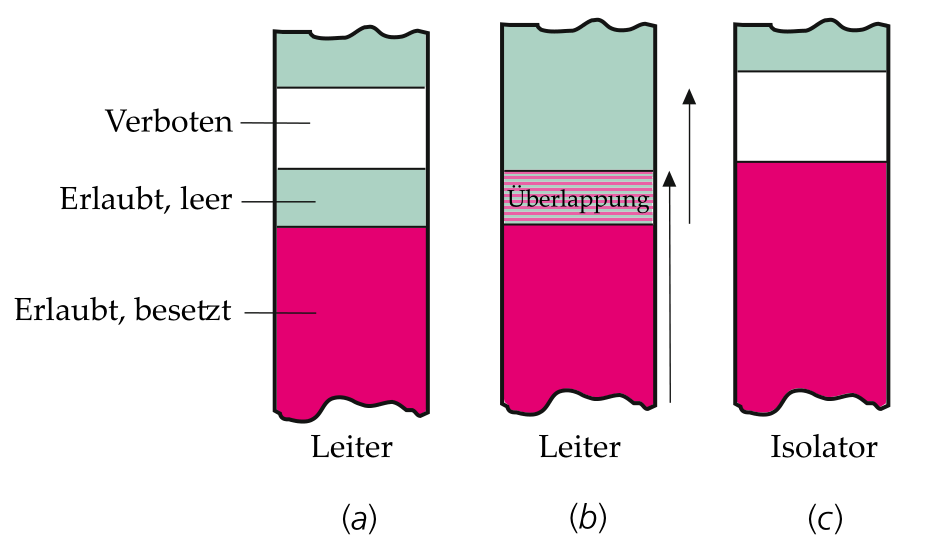
\includegraphics[width=10cm]{Bandstrukturen}
\centering
\caption{Bandstrukturen von Festkörpern. a: Ein typischer Leiter: Das Valenzband ist gleichzeitig das Leitungsband. b: Ein Leiter, bei dem das Valenzband das darüberliegende Leitungsband überlappt. c: Ein typischer Isolator: Das gefüllte Valenzband ist durch eine breite Bandlücke vom Leitungsband getrennt. \cite{tipler}}
\centering
\label{fig:bandstrukturen_leiter-isolator}
\end{figure}

\subsection{Halbleiter}
Halbleiter haben eine eher große Bandlücke, die das Valenzband von dem Leitungsband trennt.
Die Elektronen benötigen also eine bestimme Energie um die Bindung zu verlassen und als freie Ladungsträger zu agieren. \cite{werk}
Die fehlenden Elektronen im Valenzband werden Defektelektronen oder Löcher genannt. Sie verhalten sich wie positive Teilchen. \cite{hering}
Sowohl die Bewegung des freien Elektrons sowie die Bewegung des Lochs tragen zur Leitfähigkeit bei.

\subsubsection{Dotierung}
Um die nötige Energie, die die Elektronen benötigen zu verringern, werden Halbleiter dotiert. Dabei werden andere Atome mit mehr oder weniger Valenzelektronen als das Wirtsgitter in den Halbleiter eingebracht. 
Die zusätzlichen Elektronen lassen sich leichter lösen als die Bildungselektronen und die "fehlenden" Elektronen begünstigen die Entstehung von Löchern. Dies liegt daran, dass das bei der n-Dotierung das Donatorniveau durch die zusätzlichen Elektronen näher am Leitungsband liegt und Elektonen weniger Energie brauchen, um in den freien Zustand zu gelangen. \cite{werk}

\begin{figure}[H]
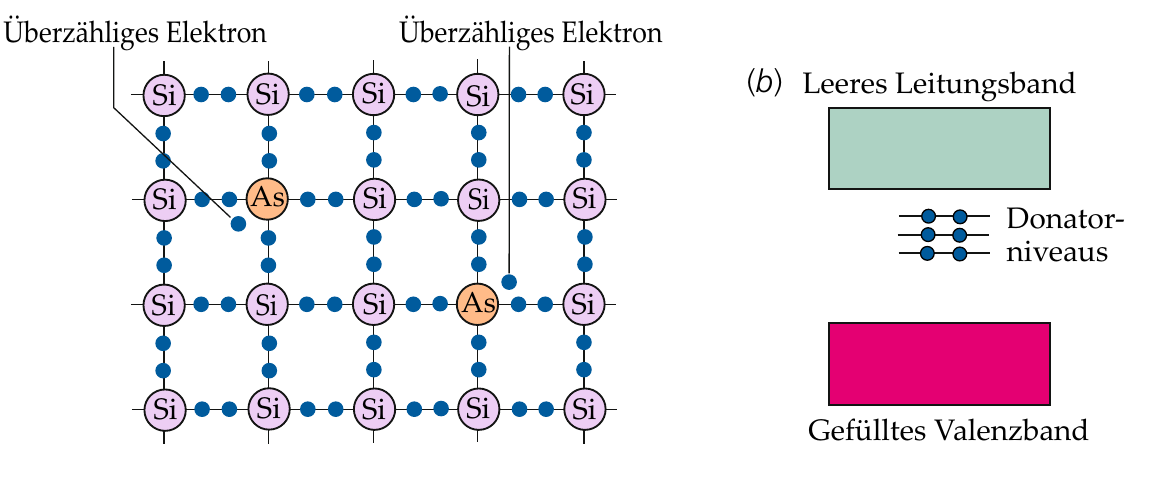
\includegraphics[width=12cm]{n-dotierter_Halbleiter}
\centering
\caption{Bandstruktur eines n-Dotierten Halbleiters \cite{tipler}}
\centering
\label{fig:bandstruktur-n-dotiert}
\end{figure}

Genauso liegt bei der p-Dotierung das Akzeptorniveau aufgrund des fehlendes Valenzelektron näher am Valenzband, wodurch auch hier weniger Energie für die Entstehung von Löchern benötigt wird. \cite{werk}

\begin{figure}[H]
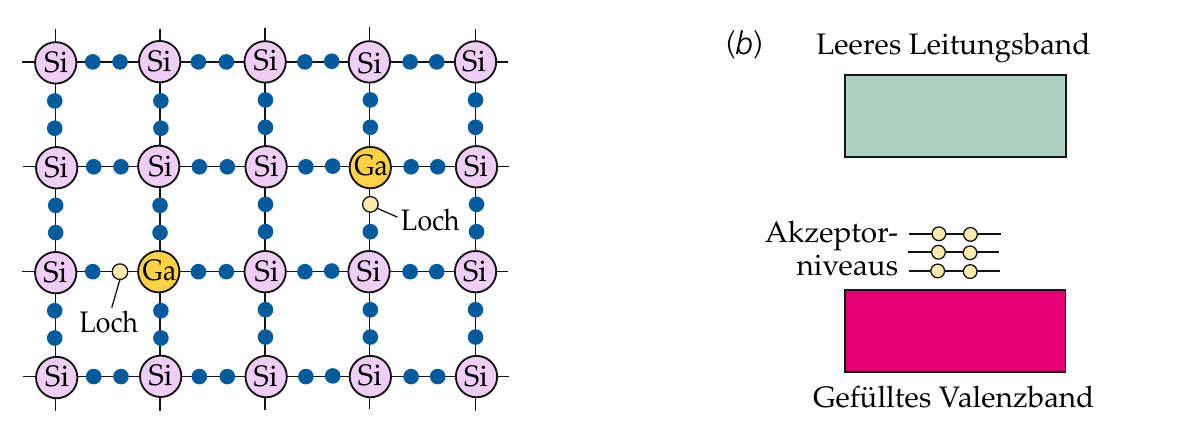
\includegraphics[width=12cm]{p-dotierter_Halbleiter}
\centering
\caption{Bandstruktur eines p-Dotierten Halbleiters \cite{tipler}}
\centering
\label{fig:bandstruktur-p-dotiert}
\end{figure}


\subsection{Messung Spezifischer Widerstand nach van der Pauw}
Mit dem Verfahren nach van der Pauw kann der Flächenwiderstand $R_{\square}$ einer dünnen, planparallelen Platte fast beliebiger Form zu bestimmt werden. Der Flächenwiderstand einer dünnen, planparallelen Platte der Dicke $d$ ist der spezifische Widerstand $\rho$ dividiert durch die Dicke der Platte. 

\begin{align}
R_{\square} = \frac{\rho}{d}
\end{align}

Somit lässt sich das Verfahren nutzen um den Spezifischen Widerstand eines Materials beliebiger Form zu messen. \cite{anl}
Das Verfahren wird gegenüber der Vierspitzenmessmethode Messmethode bevorzugt, da es den spezifischen Widerstand eine 2D-Fläche und nicht in eine lineare Richtung misst. \cite{phyglob} \\

Zur Durchführung der Messung werden vier sehr kleine Kontakte am äußeren Rand der zu messenden Probe angebracht (Abbildung 1). Die Probe muss hierbei auf ihrer gesamten Fläche die gleiche Dicke d haben und darf keine Löcher bzw. isolierte Bereiche in ihrem Inneren aufweisen. \cite{anl} \\

Anschließend wird über die Kontakte A und B ein konstanter Strom I eingeprägt und die Spannung über C und D gemessen. Daraus berechnet sich der charakteristische Widerstand: \cite{phyglob}

\begin{align}
R_{AB,DC} = \frac{U_{DC}}{I_{AB}}
\end{align}

Darauf wird dementsprechend in Strom über die Kontakte B und C eingeprägt und die Spannung über A und D gemessen. Darus ergibt sich der Widerstand $R_{BC,AD}$ \cite{anl} \\

Mit den beiden Widerständen lässt sich anschließend nach van der Pauw der Flächenwiderstand berechnen. \cite{anl}

\begin{align}
R_{\square} = \frac{\pi}{ln(2)} \cdot \frac{(R_{AB,DC}+R_{BC,AD})}{2} \cdot f(x)
\end{align}

Dabei ist $f(x)$ der Geometriefaktor (Korrekturfaktor) der entsprechend der Quelle \cite{anl} vereinfacht wie folgt berechnet wird. Dabei sind $x$ und $z$ Hilfsgrößen zur Berechnung.

\begin{align}
x = \frac{R_{AB,DC}}{R_{BC,AD}}
\end{align}

\begin{align}
z = \frac{ln(2)}{2} \cdot \left(\frac{x-1}{x+1}\right)^2
\end{align}

\begin{align}
f(x) = 1 - z - \left( 1-\frac{ln(2)}{3}\right)  \cdot z^2 - \left( 2 - \frac{4}{3} \cdot ln(2) + \frac{8}{45} \cdot ln^2(2)\right) \cdot z^2
\end{align}

\subsection{Halleffekt}
Der Halleffekt basiert grundsätzlich auf der Lorentzkraft, welche auf die Elektronen in einem, im Magnetfeld befindlichen, Halbleiter wirkt.

\subsubsection{Lorentzkraft}
Ladungsträger, die sich mit einer Geschwindigkeit $\overrightarrow{v}$ durch ein Magnetfeld $\overrightarrow{B}$ bewegen, werden durch die Lorentzkraft abgelenkt. 
Die Richtung der Lorentzkraft $\overrightarrow{F_L}$ hängt von der Ladung der Ladungsträger $q$, deren Bewegungsrichtung $\overrightarrow{v}$ und der Richtung des Magnetfeldes bzw. der Flussdichte $\overrightarrow{B}$ ab. \cite{anl}

\begin{align}
\overrightarrow{F_L} = q \cdot (\overrightarrow{v} \times \overrightarrow{B})
\end{align}

\subsubsection{Berechnung der Hall-Spannung}

Durch die Ablenkung der Elektronen im Magnetfeld entsteht auf der linken Seite des Halbleiters ein Überschuss an Elektronen, sie lädt sich negativ auf. Auf der Gegenseite verbleibt die positive Ladung der ortsfesten Donatoren. Durch die Ladungsdifferenz entsteht in dem Leiter ein elektrisches Feld. Dieses Feld lässt eine entgegengesetzte Kraft $\overrightarrow{F_H}$ auf die Elektronen wirken. Durch das Gleichsetzen dieser beiden Kräfte, lässt sich die Stärke des Feldes, bzw. die Hallspannung $U_H$ berechnen. \cite{anl}

\begin{align}
\overrightarrow{F_H} &= -\overrightarrow{F_L} \\
\overrightarrow{E_H} \cdot q &= -(q \cdot (\overrightarrow{v} \times \overrightarrow{B})) \\
\frac{U_H}{b} &= v \cdot B \text{(für $v \perp B$)}
\end{align}

\begin{align}
\Rightarrow U_H = v \cdot B \cdot b
\end{align}

Die Driftgeschwindigkeit der Elektronen, welche ausschlaggebend für die Lorentzkraft ist, ergibt sich aus der Stromdichte in dem Halbleiter. \cite{anl}

\begin{align}
j = \frac{I}{b \cdot d} \quad \text{und} \quad j = n \cdot q \cdot v
\end{align}

\begin{align}
\Rightarrow v = \frac{I}{n \cdot q \cdot b \cdot d}
\end{align}

Die beiden Gleichungen ineinander eingesetzt ergibt als Hallspannung:

\begin{align}
U_H = \frac{1}{n \cdot q} \cdot \frac{I \cdot B}{d}
\end{align}

Dabei ist der Faktor $A_H = \frac{1}{n \cdot q}$, auch Hall-Koeffizient, welcher auch über die Art der Ladungsträger aussagt. Der Hall-Koeffizient ist positiv für Löcherleitung $(q = +e)$ und negativ für Elektronenleitung $(q = -e)$. \cite{anl}

\subsubsection{Messung der Hallspannung}

Bei der Messung der Hallspannung muss bedacht werden, dass keine Probe perfekt symmetrisch ist und somit auch eine Querspannung anliegt, auch ohne das Vorhandensein eines äußeren Magnetfeldes. Die Hallspannung UH ist die Differenz zwischen Querspannung mit und ohne Magnetfeld. \cite{anl}

\begin{align}
U_H = U_{BD,\text{mit}} - U_{BD,\text{ohne}}
\end{align}


\newpage

\section{Versuch 3.1 Spezifischer Widerstand und Halleffekt}
\subsection{Häusliche Vorarbeit}
\subsubsection{3.3.2 - Van der Pauw Widerstandsnetzwerk}
Die Probe besteht aus einer Art Gitter aus Widerständen. Dabei ist jeder Punkt, der Probe nach links, rechts, oben, unten mit einem benachbarten Punkt über einen Widerstand vernetzt. Dabei kann man sich einen Widerstand im Netzwerk ersatzweise als spezifischen Widerstand des Materials vorstellen. Nach folgendem Aufbau verteilt sich der Strom auf die verschiedenen Widerstände. Dabei fließt durch die Widerstände auf der direkten Strecke zwischen VCC und GND der Hauptanteil des Stromes und je weiter man nach rechts kommt immer weniger. Dennoch wird auch an den äußeren Widerständen zwischen B und C ein messbarer Spannungsabfall erzeugt.

\begin{figure}[H]
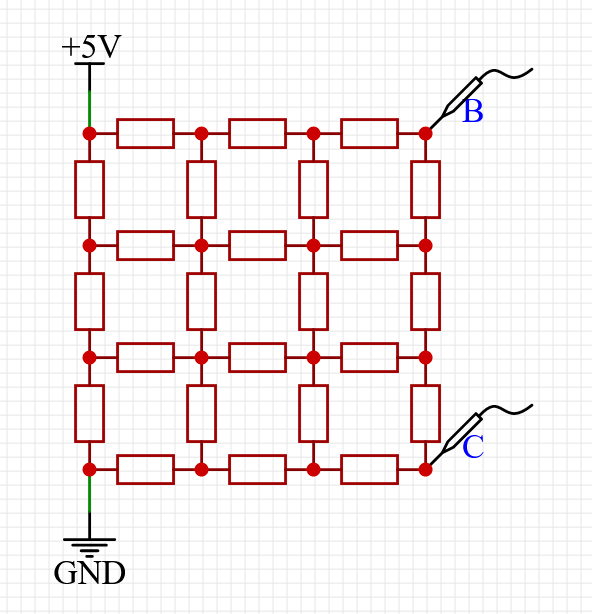
\includegraphics[width=7cm]{Widerstandsnetzwerk_v3}
\centering
\caption{Widerstandsnetzwerk bei der van der Pauw Messung}
\centering
\label{fig:widerstandsnetzwerk}
\end{figure}

Die folgende Grafik zeigt die Stromdichteverteilung in dem Netzwerk, dabei kann man an den eigezeichneten Potentiallinien erkennen, welche Spannung an B und C gemessen wird, wenn der Strom von A nach D fließt.

\begin{figure}[H]
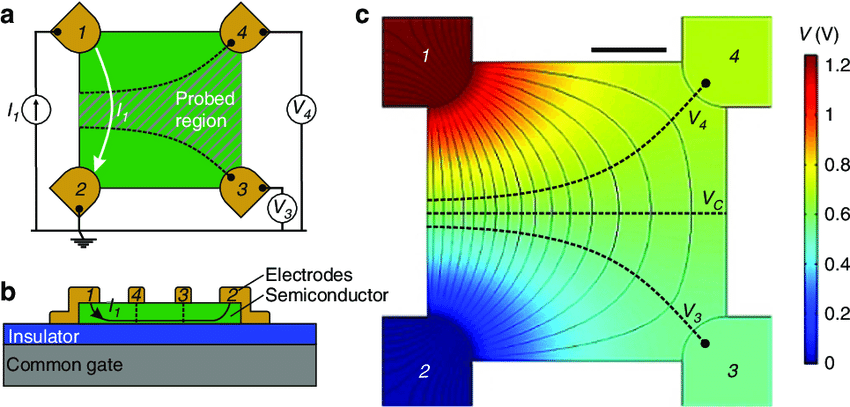
\includegraphics[width=12cm]{Top-view-of-van-der-Pauw-square-shaped}
\centering
\caption{Stromdichteverteilung bei der van der Pauw Messung \protect\footnotemark}
\centering
\label{fig:top-view-of-van-der-pauw}
\end{figure}

\footnotetext{\url{https://www.researchgate.net/figure/The-gated-van-der-Pauw-method-a-Top-view-of-a-van-der-Pauw-device-with-square-shaped_fig4_316052617}}

\subsubsection{3.3.3 - Zeichnung zum Halleffekt im p-Halbleiter}
Die folgende Abbildung zeigt alle Felder, Spannungen und Ströme für einen p-Halbleiter.

\begin{figure}[H]
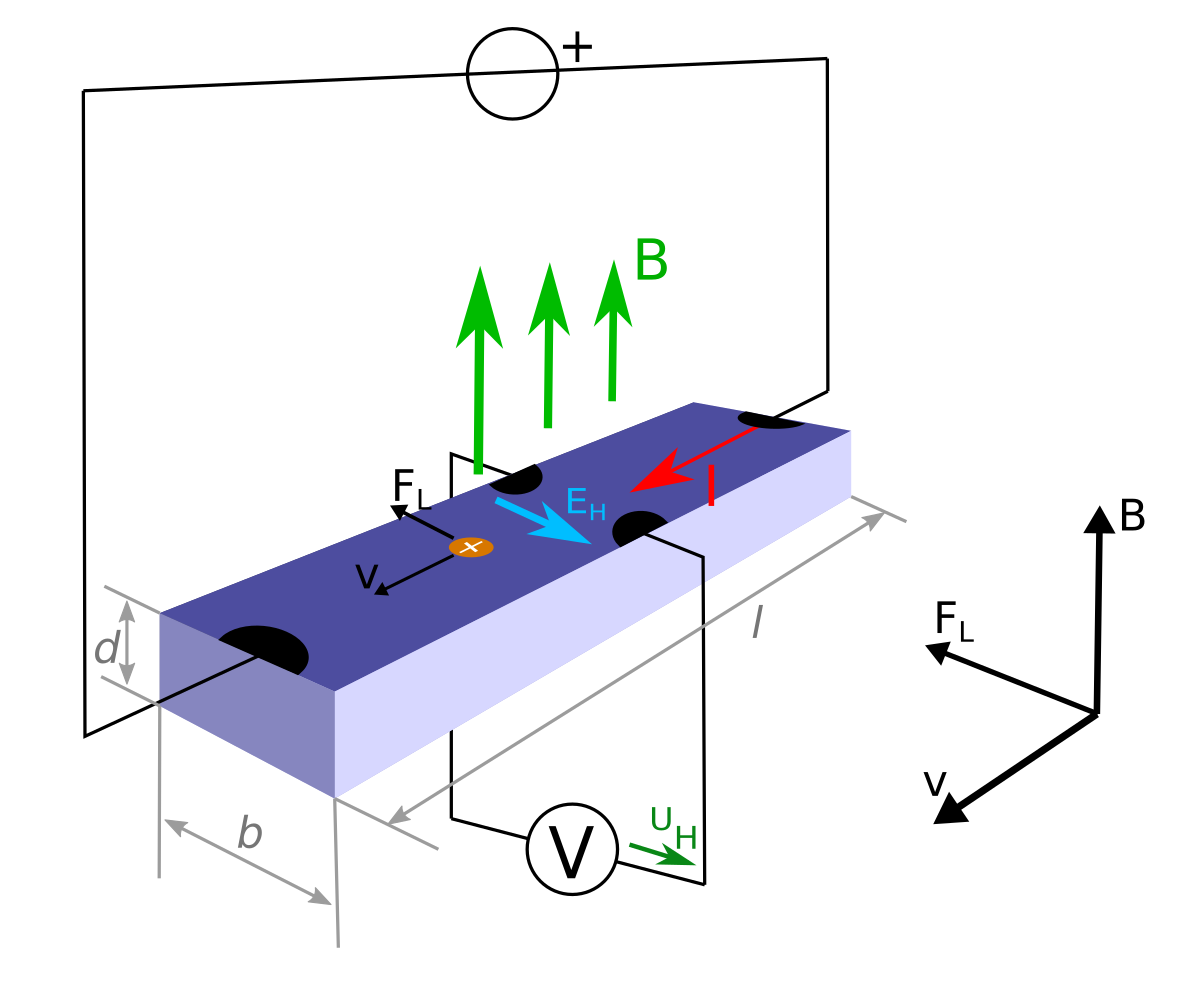
\includegraphics[width=12cm]{p-Halbleiter_Hall-Effekt}
\centering
\caption{Halleffekt im p-Halbleiter}
\centering
\label{fig:halleffekt-p-halbleiter}
\end{figure}

\subsubsection{3.3.4 - Ladungsträgerdichte von Silizium}
In den Beispielaufgaben zum der Ladungsträgerdichte von Silizium werden in dem Arbeitsbuch "Physik für Studierende der Naturwissenschaften und Technik" (vgl. \cite{tipler}) $5 \cdot 10^{16} \frac{\text{Elektronen}}{cm^3}$ als typische Werte angenommen. Dies stimmt auch mit dem in der folgenden Grafik (Abbildung~\ref{fig:spezifischer-widerstand-silizium}) markierten Bereich überein.

\subsubsection{3.3.5 - Abhängigkeit des spezifischer Widerstands von der Dotierung}
Die folgende Grafik (Abbildung~\ref{fig:spezifischer-widerstand-silizium}) zeigt die Abhängigkeit des spezifischen Widerstands in Silizium von der Dotierung. 
Dabei lässt sich ein größtenteils linearer Zusammenhang erkennen, wobei der Widerstand eines p-Dotierten Halbleiters leicht größer ist.

\begin{figure}[H]
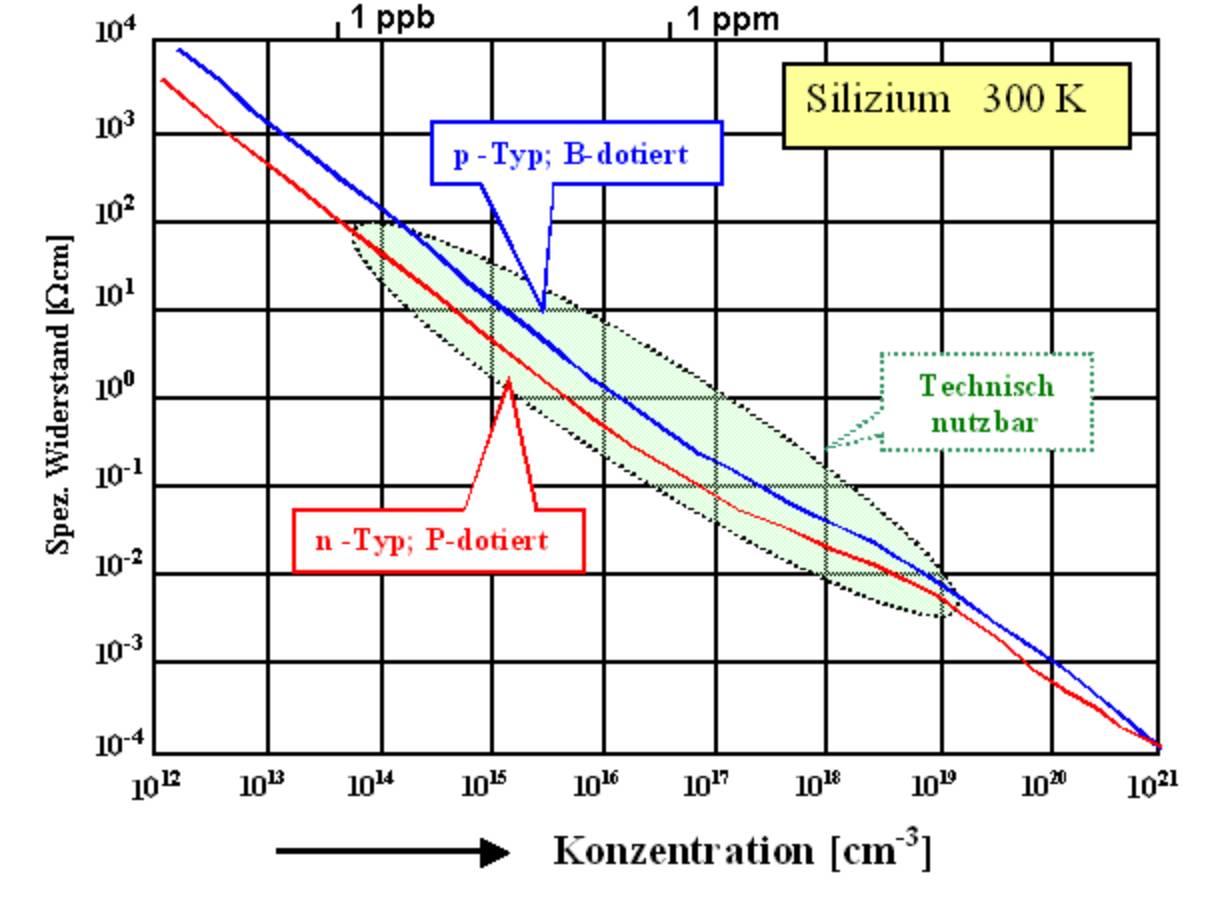
\includegraphics[width=12cm]{spezifischer_Widerstand_Silizium}
\centering
\caption{Abhängigkeit des spezifischer Widerstands von der Dotierung \protect\footnotemark}
\centering
\label{fig:spezifischer-widerstand-silizium}
\end{figure}

\footnotetext{\url{https://www.tf.uni-kiel.de/matwis/amat/mw2_ge/kap_5/backbone/r5_3_1.html}}

\subsubsection{3.3.6 - Abhängigkeit der Beweglichkeit der Elektronen / Löcher von der Dotierung}
Die folgende Abbildung zeigt die Beweglichkeit als Funktion der Elektronen–Konzentration in Ge, Si, GaAs bei Raumtemperatur. Dabei ist zu erkennen, dass die Beweglichkeit der Elektronen (in rosa) höher ist, als die der Löcher (in hellblau)

\begin{figure}[H]
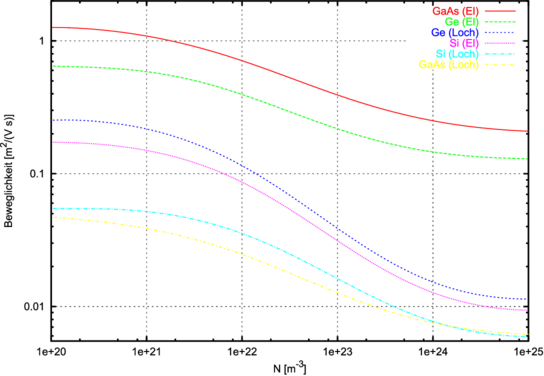
\includegraphics[width=12cm]{beweglichkeit-Silizium}
\centering
\caption{Beweglichkeit als Funktion der Elektronen–Konzentration in Ge, Si, GaAs bei Raumtemperatur \protect\footnotemark}
\centering
\label{fig:beweglichkeit-silizium}
\end{figure}

\footnotetext{\url{http://wwwex.physik.uni-ulm.de/lehre/physikalischeelektronik/phys_elektr/phys_elektrse10.html}}

\subsubsection{3.3.7 - Richtung des Magnetfelds eines Stabmagneten}
Die folgende Grafik zeigt die Feldlinien eines Stabmagneten. Dabei gehen die Feldlinien senkrecht aus dem (roten) Nordpol hervor und gehen danach wieder senkrecht in den Südpol (grün) herein.

\begin{figure}[H]
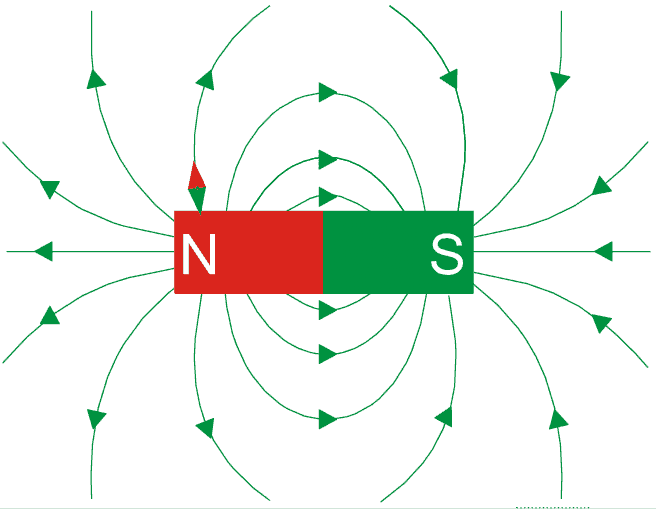
\includegraphics[width=8cm]{stabmagnet}
\centering
\caption{Magnetfelds eines Stabmagneten \protect\footnotemark}
\centering
\label{fig:stabmagnet}
\end{figure}

\footnotetext{\url{https://www.leifiphysik.de/elektrizitaetslehre/permanentmagnetismus/grundwissen/magnetfeld-und-feldlinien}}

\newpage

\subsection{Aufbau und Durchführung}
\subsubsection{Teil A: Bestimmung des spezifischen Widerstands}

Die Messschaltung wird wie in der folgenden Schaltung aufgebaut. (Abbildung~\ref{fig:messchaltung-spezifischer-widerstand})
Dazu wird der Probenhalter mit der Si-Prode (Abbildung~\ref{fig:probehalter-mit-si}) in die Messbox (Abbildung~\ref{fig:messbox-mit-anschluss}) eingebaut und die Messgeräte entsprechend des Schaltplanes angeschlossen.

\begin{figure}[H]
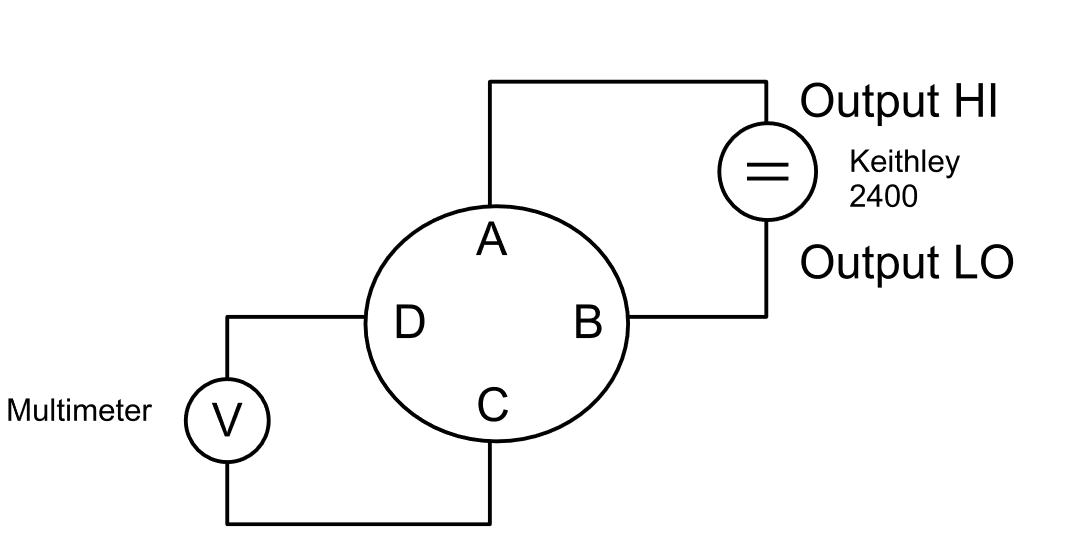
\includegraphics[width=12cm]{messchaltung_spezifischer_Widerstand}
\centering
\caption{Messschaltung zur Bestimmung des spezifischen Widerstandes \cite{anl}}
\centering
\label{fig:messchaltung-spezifischer-widerstand}
\end{figure}

\begin{figure}[H]
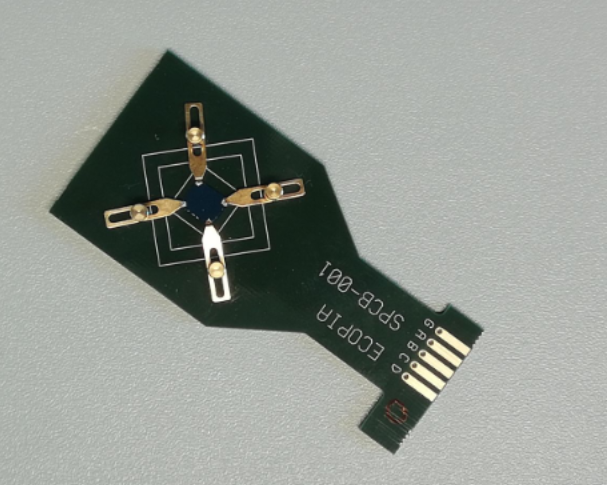
\includegraphics[width=7cm]{probehalter-mit-si}
\centering
\caption{Probenhalter mit montierter Si-Probe \cite{anl}}
\centering
\label{fig:probehalter-mit-si}
\end{figure}

\begin{figure}[H]
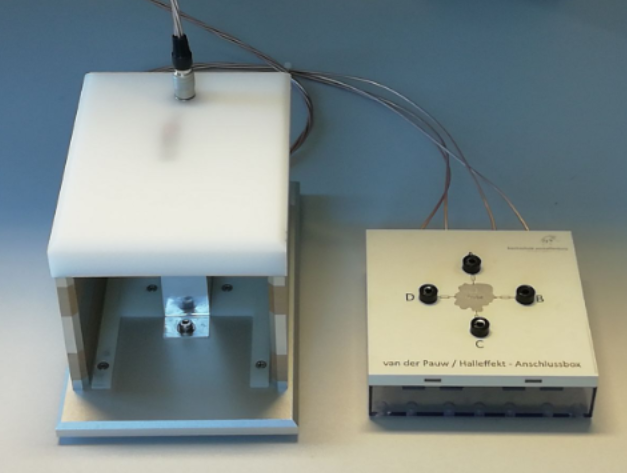
\includegraphics[width=7cm]{messbox_mit_anschluss}
\centering
\caption{Messbox mit Anschlussbox \cite{anl}}
\centering
\label{fig:messbox-mit-anschluss}
\end{figure}

Nun wird der spezifische Widerstand wie bereits in dem Theorieteil beschrieben gemessen.
Dazu wird für verschiedene Ströme (zuerst über A nach B dann über B nach C) die Spannung über D-C bzw. A-D gemessen.
Mit der Dicke der Probe lässt sich nun der spezifische Widerstand gemessen.

\subsubsection{Teil B: Bestimmung der Art der Ladungsträger}

Die Probe wird aus der Messbox entfernt und die Hallspannung wie in (Abbildung~\ref{fig:messchaltung-hall}) gemessen, während einmal der Nordpol und einmal der Südpol darüber gehalten wird. Eine Messung ohne Magnet erlaubt es den Drift (siehe Theorieteil) aus den Ergebnissen zu eliminieren.

\begin{figure}[H]
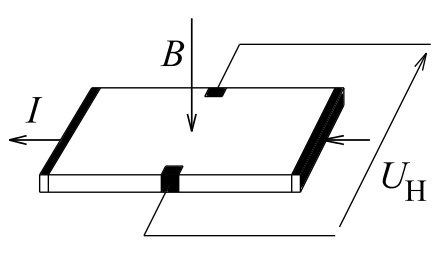
\includegraphics[width=8cm]{messchaltung_hall}
\centering
\caption{Messschaltung zur Bestimmung der Hall-Spannung \protect\footnotemark}
\centering
\label{fig:messchaltung-hall}
\end{figure}

\footnotetext{\url{https://de.wikipedia.org/wiki/Hall-Sensor}}

Die Messungen werden an einer p-Dotierten und einer n-Dotierten Germaniumprobe wiederholt und mit der Siliziumprobe, zu welcher die Dotierung unbekannt ist verglichen. Daraus lässt dich die Dotierung der Si-Probe bestimmen.

\subsubsection{Teil C: Bestimmung der Ladungsträgerdichte und Beweglichkeit}

Der Messadapter (weißer Kunststoffdeckel) mit eingebautem Probenhalter wieder vorsichtig in die Messbox eingebaut.
Anschließend wird die Hallspannung mit Dauermagnet (von forne und von hinten eingeschoben) gemessen.
Eine Messung ohne Magnet soll wieder den Drift kompensieren.\\

Anschließend wird für beide Zustände des Magneten das Magnetfeld gemessen. \\

Aus den Messergebnissen lässt sich die Ladungsträgerdichte und Beweglichkeit berechnen.

\newpage

\subsection{Auswertung Versuch}
Alle Messwerte wurden mit Excel wie folgt berechnet:\\
Mittelwerte:
\begin{align}
=\text{RUNDEN}(\text{MITTELWERT}(...);\text{Anzahl Nachkommastellen})
\end{align}
Messunsicherheit:
\begin{align}
=\frac{\text{STABW.S}(...)}{\text{WURZEL}(\text{ANZAHL}(...))} \cdot k
\end{align}
mit
\begin{align*}
k \quad &\text{Erweiterungsfaktor} = 2&\\
\end{align*}
Messunsicherheiten werden immer auf zwei signifkante Stellen aufgerundet.
\subsubsection{Teil A: Bestimmung des spezifischen Widerstands}
\paragraph{Messwerte $I_{AB}$ :\\}
Die Messwerte für die verschiedenen Hallspannungen bei den verschiedenen Strömen von A nach B werden in folgender Tabelle dargestellt.

\begin{figure}[H]
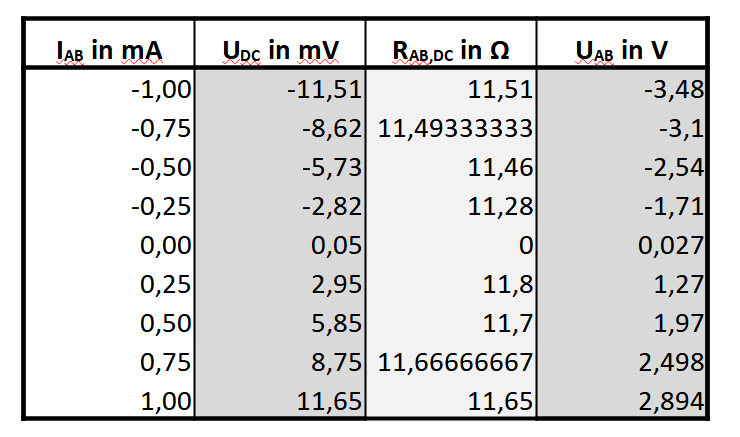
\includegraphics[width=8cm]{tabelle_messwerte_Iab}
\centering
\caption{Messwerte für Strom $I_{AB}$}
\centering
\label{fig:tabelle-messwerte-Iab}
\end{figure}

Daraus ergeben sich die Diagramme:

\begin{figure}[H]
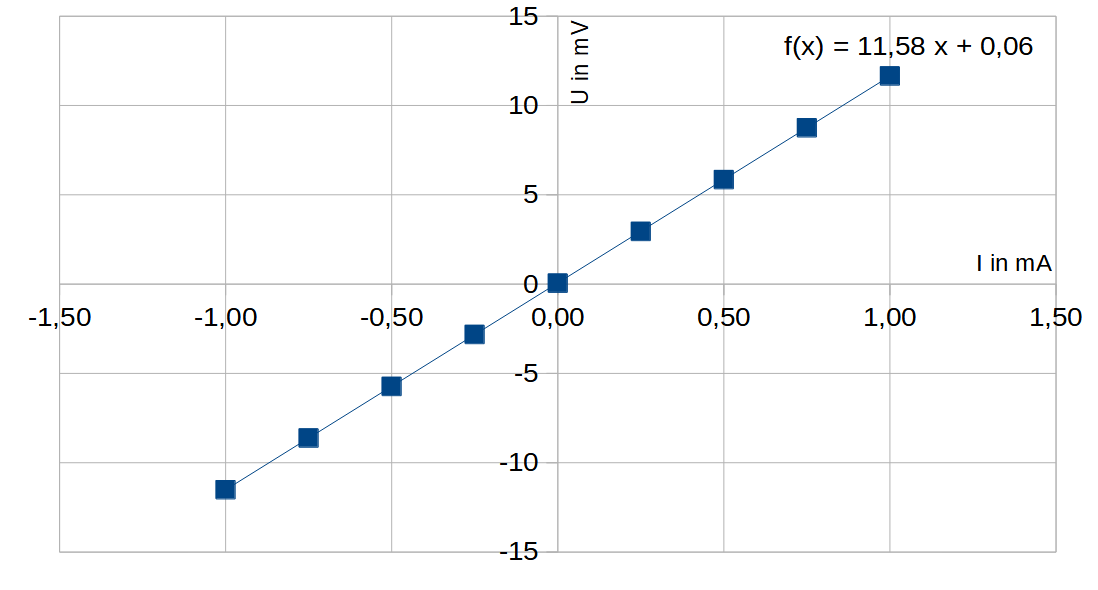
\includegraphics[width=10cm]{diagramm_messwerte_Iab-Udc}
\centering
\caption{Diagramm für $U_{DC}$ von $I_{AB}$}
\centering
\label{fig:diagramm_messwerte_Iab-Udc}
\end{figure}

\begin{figure}[H]
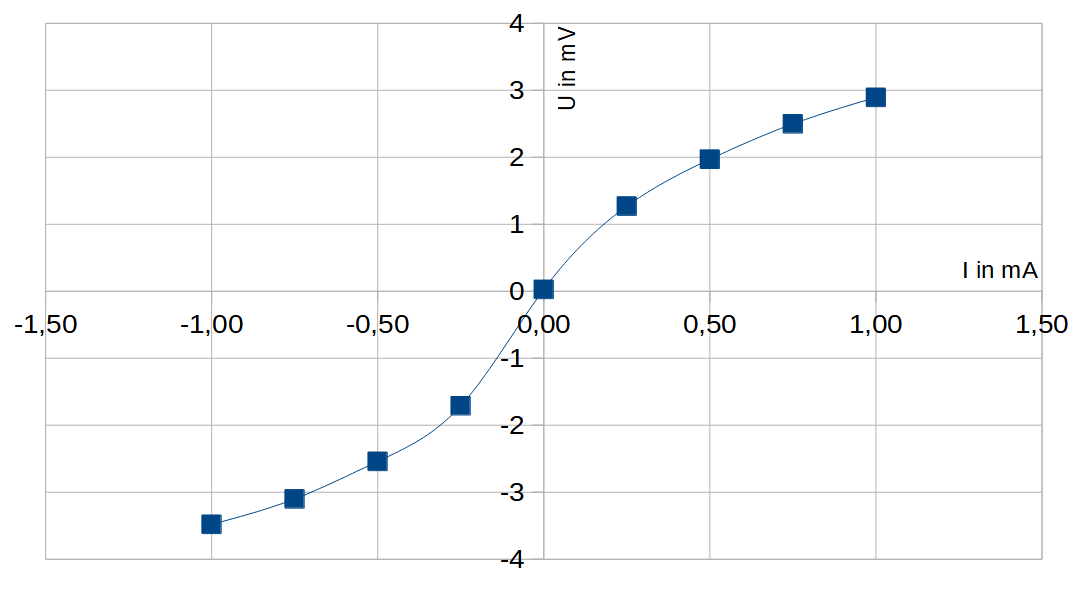
\includegraphics[width=10cm]{diagramm_messwerte_Iab-Uab}
\centering
\caption{Diagramm für $U_{AB}$ von $I_{AB}$}
\centering
\label{fig:diagramm_messwerte_Iab-Udc}
\end{figure}

Die Widerstände $R_{AB,DC}$ werden dabei wie folgt berechnet.

\begin{align}
R_{AB,DC} = \frac{U_{DC}}{I_{AB}}
\end{align}

Der Mittelwert mit Messunsicherheit beträgt dabei:

\begin{align*}
R_{AB,DC} = (11,57 \pm 0,12)\Omega
\end{align*}

\paragraph{Messwerte $I_{BC}$ :\\}
Die Messwerte für die verschiedenen Hallspannungen bei den verschiedenen Strömen von B nach C werden in folgender Tabelle dargestellt.

\begin{figure}[H]
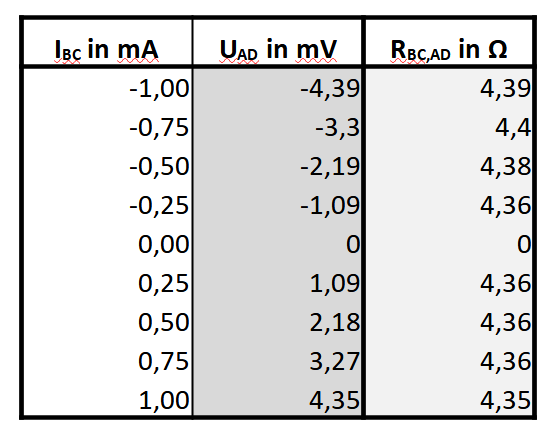
\includegraphics[width=7cm]{tabelle_messwerte_Ibc}
\centering
\caption{Messwerte für Strom $I_{BC}$}
\centering
\label{fig:tabelle-messwerte-Ibc}
\end{figure}

Daraus ergeben sich das Diagramm:

\begin{figure}[H]
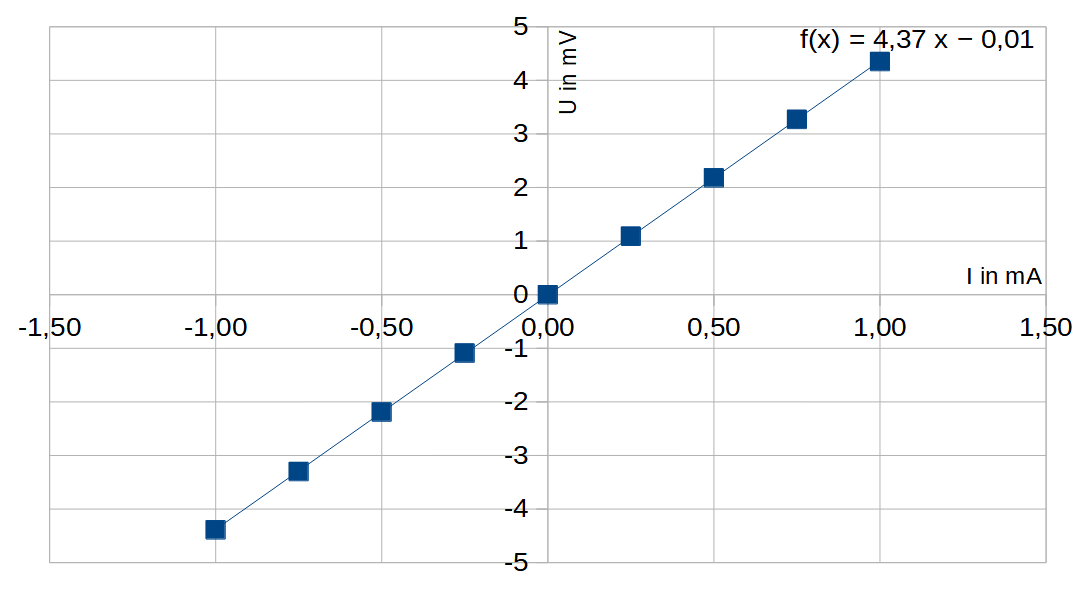
\includegraphics[width=10cm]{diagramm_messwerte_Ibc-Uad}
\centering
\caption{Diagramm für $U_{AD}$ von $I_{BC}$}
\centering
\label{fig:diagramm_messwerte_Ibc-Uad}
\end{figure}

Die Widerstände $R_{BC,AD}$ werden dabei wie folgt berechnet.

\begin{align}
R_{BC,AD} = \frac{U_{AD}}{I_{BC}}
\end{align}

Der Mittelwert mit Messunsicherheit beträgt dabei:

\begin{align*}
R_{BC,AD} = (4,37 \pm 0,13)\Omega
\end{align*}

\paragraph{Flächenwiderstand:\\}
\textbf{Mittlerer Widerstand:}\\
\begin{align}
\overline{R} = \frac{R_{AB,DC}+R_{BC,AD}}{2} = 7,97 \Omega
\end{align}
Fehlerrechnung:
\begin{align*}
\frac{\partial}{\partial R_{AB,DC}} \overline{R} &= \frac{1}{2} \\
\frac{\partial}{\partial R_{BC,AD}} \overline{R} &= \frac{1}{2}
\end{align*}
\begin{align*}
U_{\overline{R}} = \vert \frac{\partial}{\partial R_{AB,DC}} \overline{R} \vert \cdot U_{R_{AB,DC}} +  \vert \frac{\partial}{\partial R_{BC,AD}} \overline{R} \vert \cdot U_{R_{BC,AD}} = 0,125 \Omega \approx 0,13 \Omega
\end{align*}
\begin{align*}
\overline{R} = (7,97 \pm 0,13)\Omega
\end{align*}

\textbf{Erste Hilfsgröße:}\\
\begin{align}
x = \frac{R_{AB,DC}}{R_{BC,AD}} = 2,6476
\end{align}
Fehlerrechnung:
\begin{align*}
\frac{\partial}{\partial R_{AB,DC}} x &= \dfrac{1}{R_\text{BC}} \\
\frac{\partial}{\partial R_{BC,AD}} x &= -\dfrac{R_\text{AB}}{R_\text{BC}^2}
\end{align*}
\begin{align*}
U_{x} = \vert \frac{\partial}{\partial R_{AB,DC}} x \vert \cdot U_{R_{AB,DC}} + \vert \frac{\partial}{\partial R_{BC,AD}} x \vert \cdot U_{R_{BC,AD}} = 0,10622 \approx 0,11
\end{align*}
\begin{align*}
x = (2,65 \pm 0,11)
\end{align*}

\textbf{Zweite Hilfsgröße:}\\
\begin{align}
z = \frac{ln(2)}{2} \cdot (\frac{x-1}{x+1})^2 = 0,07082
\end{align}
Fehlerrechnung:
\begin{align*}
\frac{\partial}{\partial x} z = 2\ln\left(2\right)\cdot\dfrac{\left(x-1\right)}{\left(x+1\right)^3}
\end{align*}
\begin{align*}
U_{z} = \vert \frac{\partial}{\partial x} z \vert \cdot U_{x} = 0,04704 \approx 0,048
\end{align*}
\begin{align*}
z = (0,071 \pm 0,048)
\end{align*}

\textbf{Geometriefaktor:}\\
\begin{align}
f = 1 - z - \left( 1-\frac{ln(2)}{3}\right)  \cdot z^2 - \left( 2 - \frac{4}{3} \cdot ln(2) + \frac{8}{45} \cdot ln^2(2)\right) \cdot z^3 = 0,92471
\end{align}
Fehlerrechnung:
\begin{align*}
\frac{\partial}{\partial z} f = -1 -\left( 2-\frac{2\cdot ln(2)}{3}\right)  \cdot z -\left( 6 - 4 \cdot ln(2) + \frac{8}{15} \cdot ln^2(2)\right) \cdot z^2
\end{align*}
\begin{align*}
U_{f} = \vert \frac{\partial}{\partial z} f \vert \cdot U_{z} = 0,0541
\end{align*}
\begin{align*}
f = (0,925 \pm 0,055)
\end{align*}

\textbf{Flächenwiderstand:}\\
\begin{align}
R_{\square} = \frac{\pi}{ln(2)} \cdot \overline{R} \cdot f = 33,4137
\end{align}
Fehlerrechnung:
\begin{align*}
\frac{\partial}{\partial \overline{R}} R_{\square} &= \frac{\pi}{ln(2)} \cdot f \\
\frac{\partial}{\partial f} R_{\square} &= \frac{\pi}{ln(2)} \cdot \overline{R}
\end{align*}
\begin{align*}
U_{R_{\square}} = \vert \frac{\partial}{\partial \overline{R}} R_{\square}  \vert \cdot U_{\overline{R}} + \vert \frac{\partial}{\partial f} R_{\square} \vert \cdot U_{f} = 2,532 \frac{\Omega}{\square} \approx 2,6 \frac{\Omega}{\square}
\end{align*}
\begin{align*}
R_{\square} = (33,4 \pm 2,6)\frac{\Omega}{\square}
\end{align*}


\paragraph{Spezifischer Widerstand:\\}

\textbf{Probendicke:\\}
Als Probendicke wurde $0,525mm$ mit einer Messungenauigkeit von $\pm 0,01mm$ gemessen.

\textbf{Spezifischer Widerstand:}
\begin{align}
\rho = d \cdot R_{\square} = 1,7535
\end{align}
Fehlerrechnung:
\begin{align*}
\frac{\partial}{\partial d} \rho &= R_{\square} \\
\frac{\partial}{\partial R_{\square}} \rho &= d
\end{align*}
\begin{align*}
U_{\rho} = \vert \frac{\partial}{\partial d} \rho \vert \cdot U_{d} + \vert \frac{\partial}{\partial R_{\square}} \rho \vert \cdot U_{R_{\square}} = 0,1699 \Omega cm \approx 0,17
\end{align*}
\begin{align*}
\rho = (1,75 \pm 0,17)\Omega cm
\end{align*}


\subsubsection{Teil B: Bestimmung der Art der Ladungsträger}
Die folgenden Tabellen zeigen das verhalten der Hallspannungen bei verschiedenen Halbleiterproben:

\textbf{Messwerte an Siliziumprobe:\\}

\begin{figure}[H]
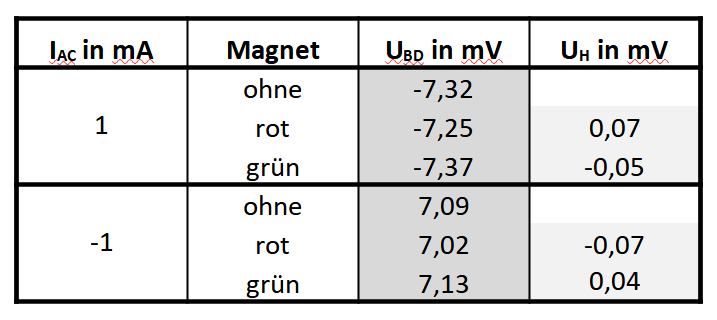
\includegraphics[width=8cm]{tabelle_messwerte_silizium}
\centering
\caption{Messwerte für Siliziumprobe}
\centering
\label{fig:tabelle_messwerte_silizium}
\end{figure}

\textbf{Messwerte an n-Germanium:\\}

\begin{figure}[H]
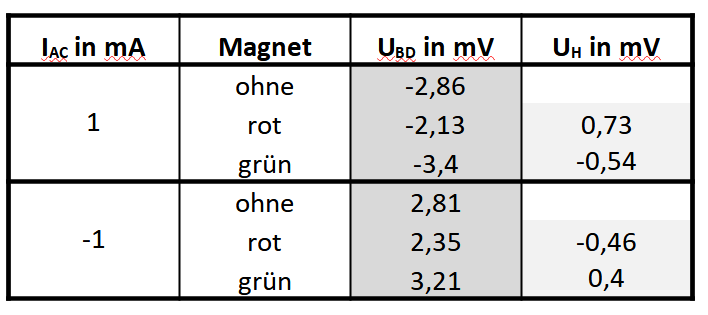
\includegraphics[width=8cm]{tabelle_messwerte_n-germanium}
\centering
\caption{Messwerte für n-Germanium}
\centering
\label{fig:tabelle_messwerte_n-germanium}
\end{figure}

\textbf{Messwerte an p-Germanium:\\}

\begin{figure}[H]
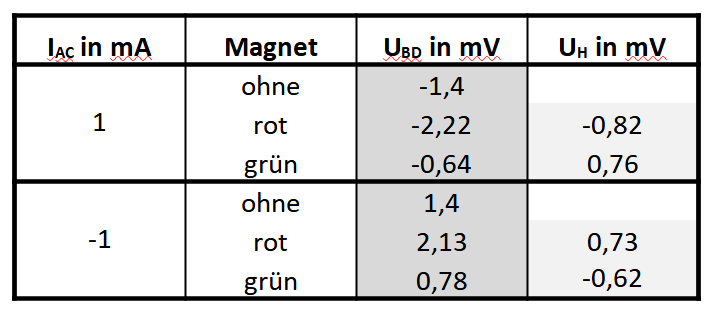
\includegraphics[width=8cm]{tabelle_messwerte_p-germanium}
\centering
\caption{Messwerte an p-Germanium}
\centering
\label{fig:tabelle_messwerte_p-germanium}
\end{figure}

Das Verhalten der unbekannten Siliziumprobe ähnelt dem der Probe des n-Dotierten Germaniums. Folglich handelt es sich bei der Probe um einen n-dotierten Siliziumhalbleiter.

\subsubsection{Teil C: Bestimmung der Ladungsträgerdichte und Beweglichkeit}

\paragraph{Hallspannung:\\}
Die Messwerte für die verschiedenen Hallspannungen bei einem Strom von $I = (1\pm0.002)mA$ werden in folgender Tabelle dargestellt.

\begin{figure}[H]
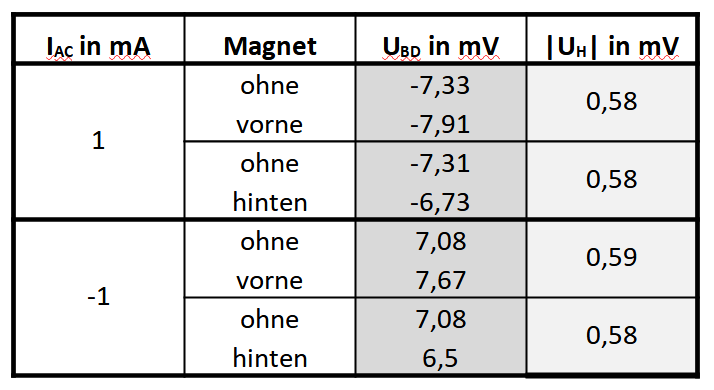
\includegraphics[width=8cm]{tabelle_messwerte_hallspannung}
\centering
\caption{Messwerte für die Hallspannung}
\centering
\label{fig:tabelle_messwerte_hallspannung}
\end{figure}

Als Mittelwert und Messungenauigkeit ergibt sich:

\begin{align*}
U_{\text{Hall}} = (0,5825\pm0,0050)mV
\end{align*}

\paragraph{Magnetfeld:\\}
Die folgende Tabelle zeigt die verschiedenen Messungen für die Stärke des Magnetfeldes.

\begin{figure}[H]
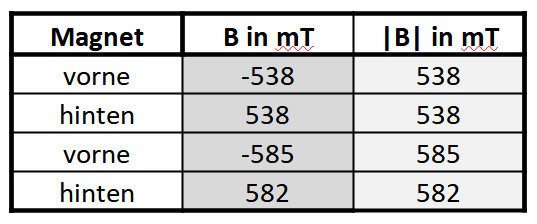
\includegraphics[width=8cm]{tabelle_messwerte_megnetfeld}
\centering
\caption{Messwerte für das Magnetfeld}
\centering
\label{fig:tabelle_messwerte_megnetfeld}
\end{figure}

Als Mittelwert und Messungenauigkeit ergibt sich:

\begin{align*}
B = (561\pm27)mT
\end{align*}

\paragraph{Ladungsträgerdichte:\\}
\begin{align}
U_H = \frac{1}{n \cdot e} \cdot \frac{I \cdot B}{d} \quad \Rightarrow \quad n = \frac{I \cdot B}{U_H \cdot e \cdot d} = 1,14568 \cdot 10^{16} \frac{1}{cm^3}
\end{align}
Fehlerrechnung:
\begin{align*}
\frac{\partial}{\partial I} n &= \frac{B}{U_H \cdot e \cdot d} \\
\frac{\partial}{\partial B} n &= \frac{I}{U_H \cdot e \cdot d} \\
\frac{\partial}{\partial U_H} n &= -\frac{I \cdot B}{U_H^2 \cdot e \cdot d} \\
\frac{\partial}{\partial d} n &= -\frac{I \cdot B}{U_H \cdot e \cdot d^2}
\end{align*}
\begin{align*}
U_{n} = \vert \frac{\partial}{\partial I} n \vert \cdot U_{I} + 
		\vert \frac{\partial}{\partial B} n \vert \cdot U_{B} +
		\vert \frac{\partial}{\partial U_H} n \vert \cdot U_{U_H} +
		\vert \frac{\partial}{\partial d} n \vert \cdot U_{d} = 0,10962 \cdot 10^{16} \frac{1}{cm^3}
\end{align*}
\begin{align*}
n = (1,15 \pm 0,11)10^{16} \frac{1}{cm^3}
\end{align*}

\paragraph{Beweglichkeit:\\}
\begin{align}
\rho = \frac{1}{e \cdot n \cdot \mu} \quad \Rightarrow \quad \mu = \frac{1}{e \cdot n \cdot \rho} = 310,137 \frac{cm^2}{Vs}
\end{align}
Fehlerrechnung:
\begin{align*}
\frac{\partial}{\partial \rho} \mu &= \frac{1}{e \cdot n \cdot \rho^2} \\
\frac{\partial}{\partial n} \mu &= \frac{1}{e \cdot n^2 \cdot \rho} 
\end{align*}
\begin{align*}
U_{n} = \vert \frac{\partial}{\partial \rho} \mu \vert \cdot U_{\rho} + 
		\vert \frac{\partial}{\partial n} \mu \vert \cdot U_{n} = 59.7928 \frac{cm^2}{Vs} \approx 60 \frac{cm^2}{Vs}
\end{align*}
\begin{align*}
\mu = (310 \pm 60)\frac{cm^2}{Vs}
\end{align*}

\newpage

\subsection{Wertung/Fazit}
Die errechneten Werte weisen kleinere Abweichung im Vergleich zu den unterschiedlichen Literaturwerten auf. Auch die Messunsicherheiten sind nicht gerade genau. Dennoch sind die gemessenen Werte in der Nähe der Literaturwerte. Dabei muss beachtetet werden, dass die Literatur nur Bereiche angibt, in welchen sich typische Werte aufhalten, und (im Falle der genutzten Literatur) keine genauen Werte gegeben sind. Dies liegt daran, da die Eigenschaften von jedem Halbleiter unterschiedlich sind, je nachdem wie dieser hergestellt wurde.
Nach der Abbildung (Abbildung~\ref{fig:spezifischer-widerstand-silizium}) ist das Ergebnis inmitten des als "technisch nutzbar" markierten Bereiches. Auch stimmen die Ladungsträgerdichte $n$ und der spezifische Widerstand $\rho$ mit einem Punkt in der Grafik überein. So sind Werte von $n \approx 1 \cdot 10^{16} \frac{1}{cm^3}$ und $\rho \approx 1 \cdot 10^0 \Omega cm$ durchaus realistisch.
Die Messungen sind keineswegs perfekt, aber bewegen sich in den realistischen Größenordnungen.

\newpage


\section{Versuch 3.2 pn-Übergang und Solarzelle}
\subsection{Häusliche Vorarbeit}
\subsubsection{An welchen Stellen des I-U Diagramms wird eine höhere Dichte an Messwerten benötigt?}
Am Anfang der Kennlinie von $-2V$ bis $0V$ ist der Verlauf relativ linear. Dadurch werden theoretisch nur
zwei Messwerte und praktisch nur wenige Messwerte benötigt. Das liegt daran, dass die Diode für diesen
Fall in Sperrrichtung geschaltet ist und die Spannung am parallelgeschalteten Widerstand $r_{\text{sh}}$
abfällt (siehe Abbildung \ref{fig:ESB_Solar}). Ab $0V$ wird die Diode nicht mehr in Sperrrichtung sondern
in Flussrichtung geschaltet, wodurch der Anteil des Stromes der durch die Diode fließt zunimmt.
Da die Kennlinie der Diode exponentiell verläuft und der größte Teil der Spannung nun an der Diode
abfällt, muss die Anzahl der Messwerte deutlich erhöht werden.

\begin{figure}[H]
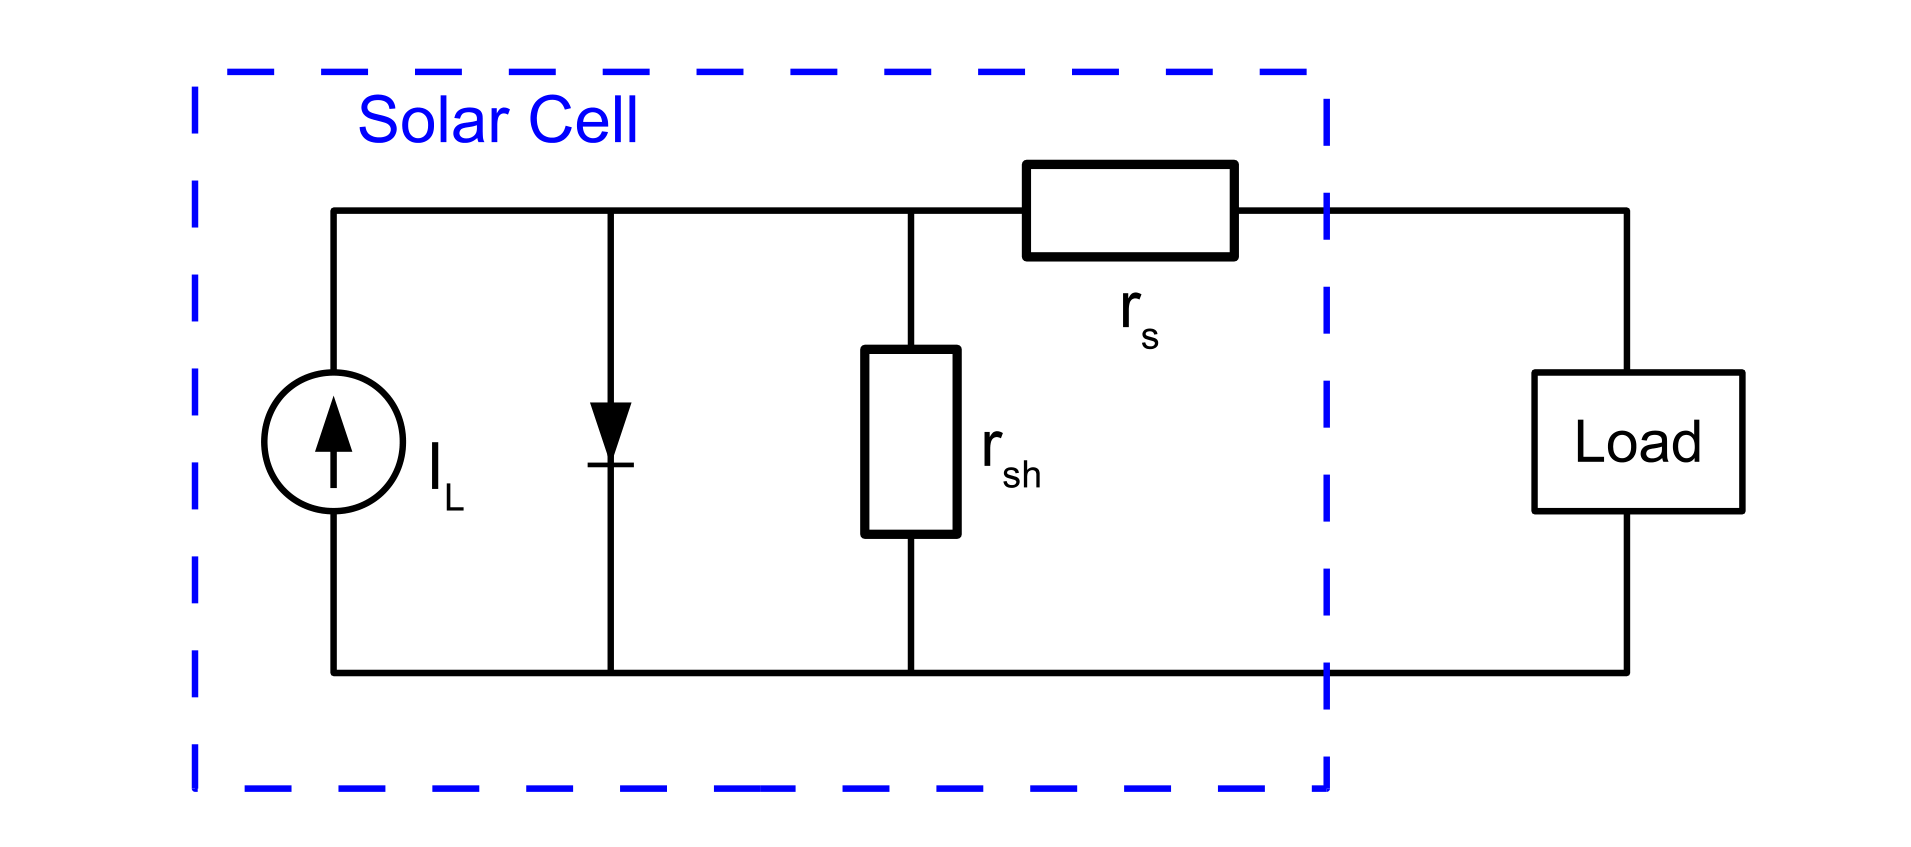
\includegraphics[width=16cm]{ESB_Solarzelle}
\centering
\caption{Ersatzschaltbild der Solarzelle \cite{anl}}
\centering
\label{fig:ESB_Solar}
\end{figure}

\subsubsection{I-U Diagramme für eine unbeleuchtete und beleuchtete Solarzelle}

\begin{figure}[H]
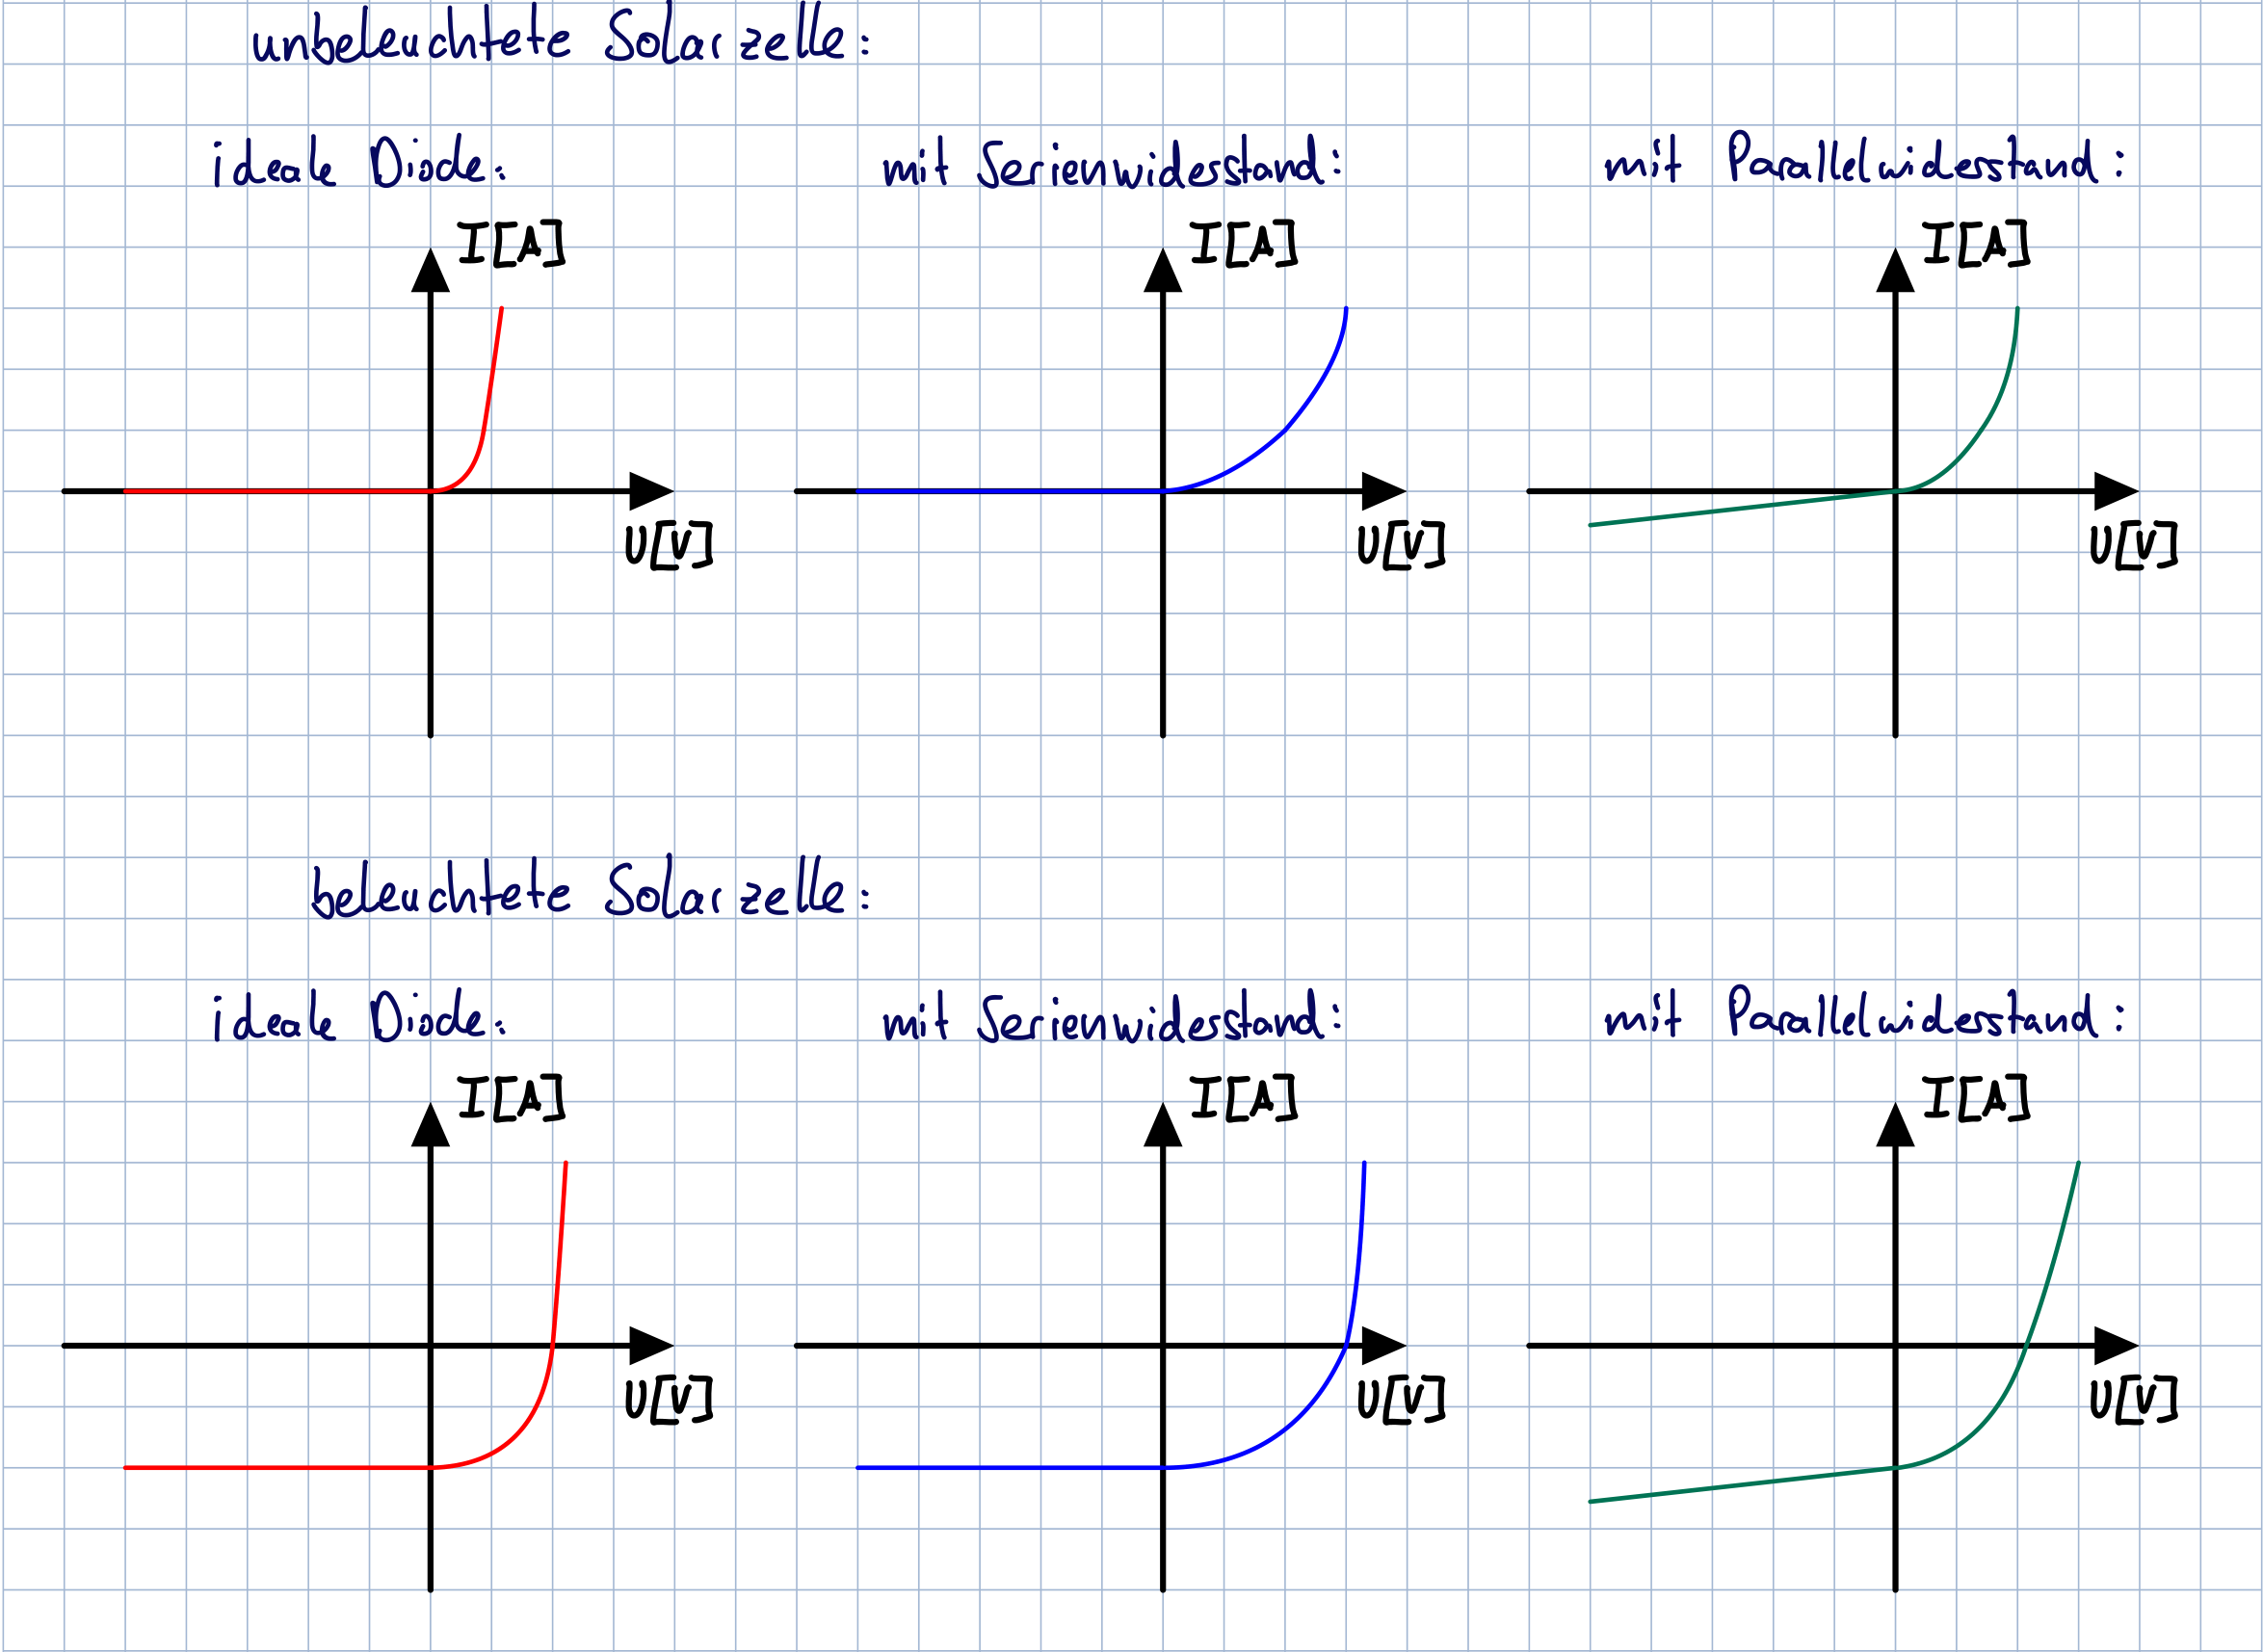
\includegraphics[width=16cm]{Kennlinie}
\centering
\caption{Kennlinien für beleuchtete und unbeleuchtete Solarzelle}
\centering
\label{fig:Kennlinien}
\end{figure}

\subsubsection{Einfluss der Widerstände auf den Füllfaktor}
Je größer der Füllfaktor wird, desto mehr ähnelt die Kennlinie einer idealen Stromquelle. Das heißt die
Solarzelle wird effizienter, je näher der Füllfaktor am Wert 1 liegt. Dies wäre der Fall, wenn
der Serienwiderstand gegen 0 $\lim_{r_{\text{s}} \to 0}$ und der Parallelwiderstand gegen unendlich ginge
$\lim_{r_{\text{sh}} \to \infty}$ (siehe Abbildung \ref{fig:ESB_Solar}).

\subsubsection{Aktueller Stand der Technik bei Solarzellen}
Solarzellen bestehen zum größten Teil aus p-dotiertem und n-dotiertem Silizium.
Es wird vor Allem wegen der hohen Verfügbarkeit auf der Erde verwendet.
Man unterscheidet zwischen polykristallinen- und monokristallinen Zellen.
Polykristalline Zellen werden aus Silizium gegossen und haben einen Wirkungsgrad
von 12-16\%. Monokristalline Zellen werden aus gezüchtetem Silizium gebaut, wodurch die Herstellung
teurer ist. Dafür wird ein höhere Effizienzvon 14-20\% erreicht. Der typische Füllfaktor liegt
zwischen 0,5 und 0,7. \cite{solar}

\newpage

\subsection{Aufbau und Durchführung}
\subsubsection{Aufbau}
Der Versuchsaufbau ist in Abbildung \ref{fig:Aufbau} dargestellt.

\begin{figure}[H]
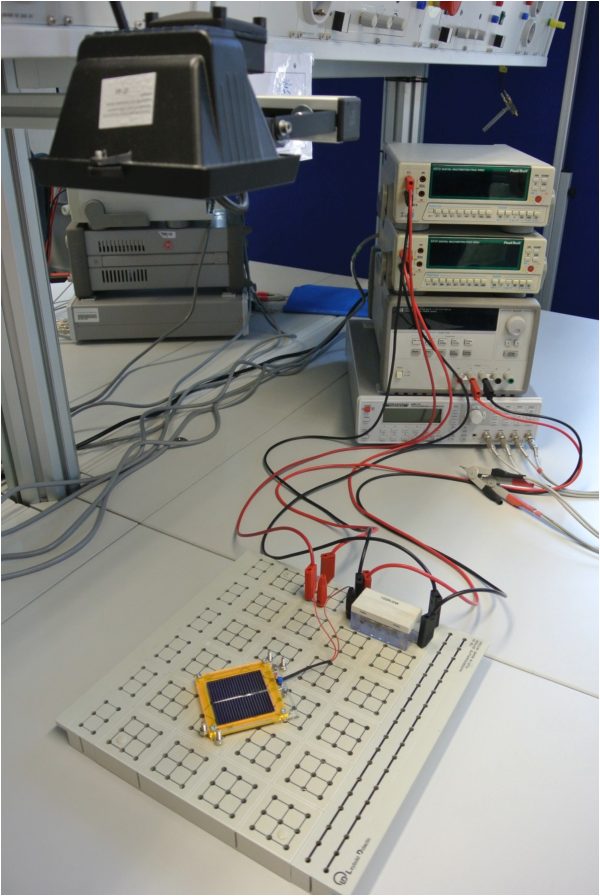
\includegraphics[width=14cm]{Aufbau}
\centering
\caption{Versuchsaufbau \cite{anl}}
\centering
\label{fig:Aufbau}
\end{figure}

\subsubsection{Durchführung}
Die Schaltung wird wie in Abbildung \ref{fig:Schaltplan} zu sehen
aufgebaut. Zuerst wird der Versuch mit abgedeckter Solarzelle durchgeführt. Man misst für verschiedene
Spannungen $U_d$ von $-2,0V$ bis $0,6V$ die Spannung $U_R$. Dadurch lässt sich der Diodenstrom $I_d$
berechnen. Mit den Strom- und Spannungswerten lässt sich nun die U-I Kennlinie der Diode zeichnen. Danach 
wird der Versuch nochmal mit beleuchteter Solarzelle wiederholt.

\begin{figure}[H]
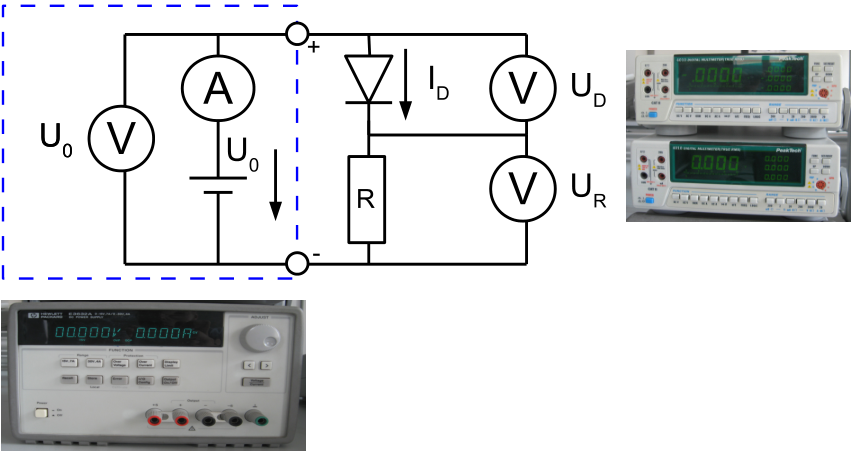
\includegraphics[width=16cm]{Schaltplan}
\centering
\caption{Schaltplan \cite{anl}}
\centering
\label{fig:Schaltplan}
\end{figure}

\newpage

\subsection{Auswertung Versuch}
Die Kapazität $C_s$ beträgt: $924,63\;nF$. Die Standardabweichung wird
auf $1\;nF$ geschätzt.

\begin{align*}
C_s = (925,0\pm 1,0)\;nF	
\end{align*}

Die Solarzelle hat eine quadratische Grundfläche $A$ mit einer Seitenlänge (l)
von $(52,5\pm 0,5)\;mm$.

\begin{align*}
A &= l^2 \\
 &= (52,5\;mm)^2 \\
 &= 2756,25\;mm^2
\end{align*}

\begin{align}
\frac{\partial A}{\partial l} = 2l
\end{align}

\begin{align*}
U_a = \bigg | \frac{\partial A}{\partial l} \bigg | \cdot U_l = 52,5\;mm^2 \\
A = (2756\pm 53)\;mm^2
\end{align*}

Die Kapazität eines Plattenkondensators mit gegebenem $\epsilon_r = 11,9$ lässt sich berechnen mit:
\begin{align*}
C &= \epsilon_0 \cdot \epsilon_r \cdot \frac{A}{d} \\
d &= \epsilon_0 \cdot \epsilon_r \cdot \frac{A}{C} \\
  &= 8,854 \cdot 10^{-12}\; \frac{As}{Vm} \cdot 11,9 \cdot \frac{2756,26 \; mm^2}{924,64 \; nF} \\
  &= 314,082 \; nm 
\end{align*}

\begin{align}
&\frac{\partial d}{\partial A} = \epsilon_0 \cdot \epsilon_r \cdot \frac{1}{C}
&\frac{\partial d}{\partial C} = - \epsilon_0 \cdot \epsilon_r \cdot \frac{A}{C^2}
\end{align}

\begin{align*}
U_d = \bigg | \frac{\partial d}{\partial A} \bigg | \cdot U_A + \bigg | \frac{\partial d}{\partial C} 
\bigg | \cdot U_C = 6,3222 \; nm
\end{align*}
\begin{align*}
d = (314,1 \pm 6,4)\; nm
\end{align*}

Folgende Größen lassen sich in der Abbildung \ref{fig:beleuchtet} oder der Tabelle \ref{tab:beleuchtet} im 
Anhang (Abschnitt \ref{sec:Anhang}) ablesen:
\begin{align*}
&\text{Die Leerlaufspannung}\; U_{OC} \; \text{beträgt:} &&0,52\;V \\
&\text{Der Kurzschulssstrom}\; I_{SC} \; \text{beträgt:} &-&0,064333\;A \\
&\text{Die maximale Leistung}\; P_{max} \; \text{beträgt:} &-&0,024296\;W\\
\end{align*}

Der Füllfaktor lässt sich durch die Gleichung berechnen:
\begin{align*}
FF = \frac{-0,024296\;W}{0,52\;V \cdot (-0,064333\;A)} = 0,72625
\end{align*}
\\
Messunsicherheit Multimeter geschätzt:
\begin{align*}
U_M = \pm 0,01\;V
\end{align*}
\begin{align*}
U_{OC} = (0,52 \pm 0,01)\;V \\
U_R = (-9,65 \pm 0,01)\;V
\end{align*}

Messunsicherheit vom Widerstand $R$:
\begin{align*}
R = (150 \pm 10)\; \Omega \\
\end{align*}

Die Messunsicherheit für $I_{SC}$ berechnet sich wie folgt:
\begin{align*}
I_{SC} = \frac{U_R}{R}
\end{align*}

\begin{align}
&\frac{\partial I_{SC}}{\partial U_R} = \frac{1}{R}
&\frac{\partial I_{SC}}{\partial R} = - \frac{U_R}{R^2}
\end{align}

\begin{align*}
U_{I_{SC}} = \bigg | \frac{\partial I_{SC}}{\partial U_R} \bigg | \cdot U_{U_R} +
\bigg | \frac{\partial I_{SC}}{\partial R} \bigg | \cdot U_R = 0,0043\overline{5} \; A
\end{align*}
\begin{align*}
I_{SC} = (-0,0643 \pm 0,0044)\; A
\end{align*}

Die Messunsicherheit für $P_{max}$ berechnet sich wie folgt:
\begin{align*}
P_{max} = U_{OC} \cdot I_{SC}
\end{align*}

\begin{align}
&\frac{\partial P_{max}}{\partial U_{OC}} = I_{SC}
&\frac{\partial P_{max}}{\partial I_{SC}} = U_{OC}
\end{align}

\begin{align*}
U_{P_{max}} = \bigg | \frac{\partial P_{max}}{\partial U_{OC}} \bigg | \cdot U_{U_{OC}} +
\bigg | \frac{\partial P_{max}}{\partial I_{SC}} \bigg | \cdot U_{I_{SC}} = 0,0029313 \; W
\end{align*}
\begin{align*}
P_{max} = (-0,0243 \pm 0,0030)\; W
\end{align*}

Die Messunsicherheit für den Füllfaktor $FF$ berechnet sich wie folgt:

\begin{align}
\frac{\partial FF}{\partial P_{max}} = \frac{1}{U_{OC} \cdot I_{SC}} \qquad
\frac{\partial FF}{\partial U_{SC}} = -\frac{P_{max}}{U_{SC}^2 \cdot I_{SC}} \qquad
\frac{\partial FF}{\partial I_{SC}} = -\frac{P_{max}}{U_{SC} \cdot I_{SC}^2}
\end{align}

\begin{align*}
U_{FF} = \bigg | \frac{\partial FF}{\partial P_{max}} \bigg | \cdot U_{P_{max}} +
\bigg | \frac{\partial FF}{\partial U_{SC}} \bigg | \cdot U_{U_{SC}} +
\bigg | \frac{\partial FF}{\partial I_{SC}} \bigg | \cdot U_{I_{SC}} = 0,1533
\end{align*}
\begin{align*}
FF = (0,73 \pm 0,16)
\end{align*}

\newpage

\subsection{Wertung/Fazit}
Der aus den Messwerten berechnete Füllfaktor liegt mit Ungenauigkeit im realistischen
Bereich. Durch die von uns sehr klein gewählte Schrittweite der Messwerte ist es uns
gelungen eine nah an der Theorie liegende U-I Kennlinie zu zeichnen.
Das Ergebnis des Versuchs ist alles in allem zufriedenstellend.

\newpage

\section{Anhang}
\label{sec:Anhang}
\begin{table}[H]
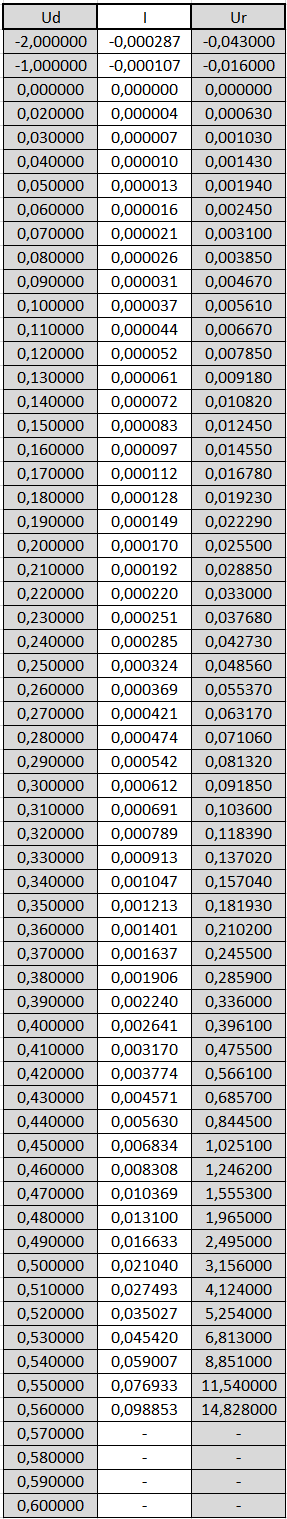
\includegraphics[width=4cm]{Tabelle_unbeleuchtet}
\centering
\caption{Messwerte Solarzelle unbeleuchtet}
\end{table}

\begin{figure}[H]
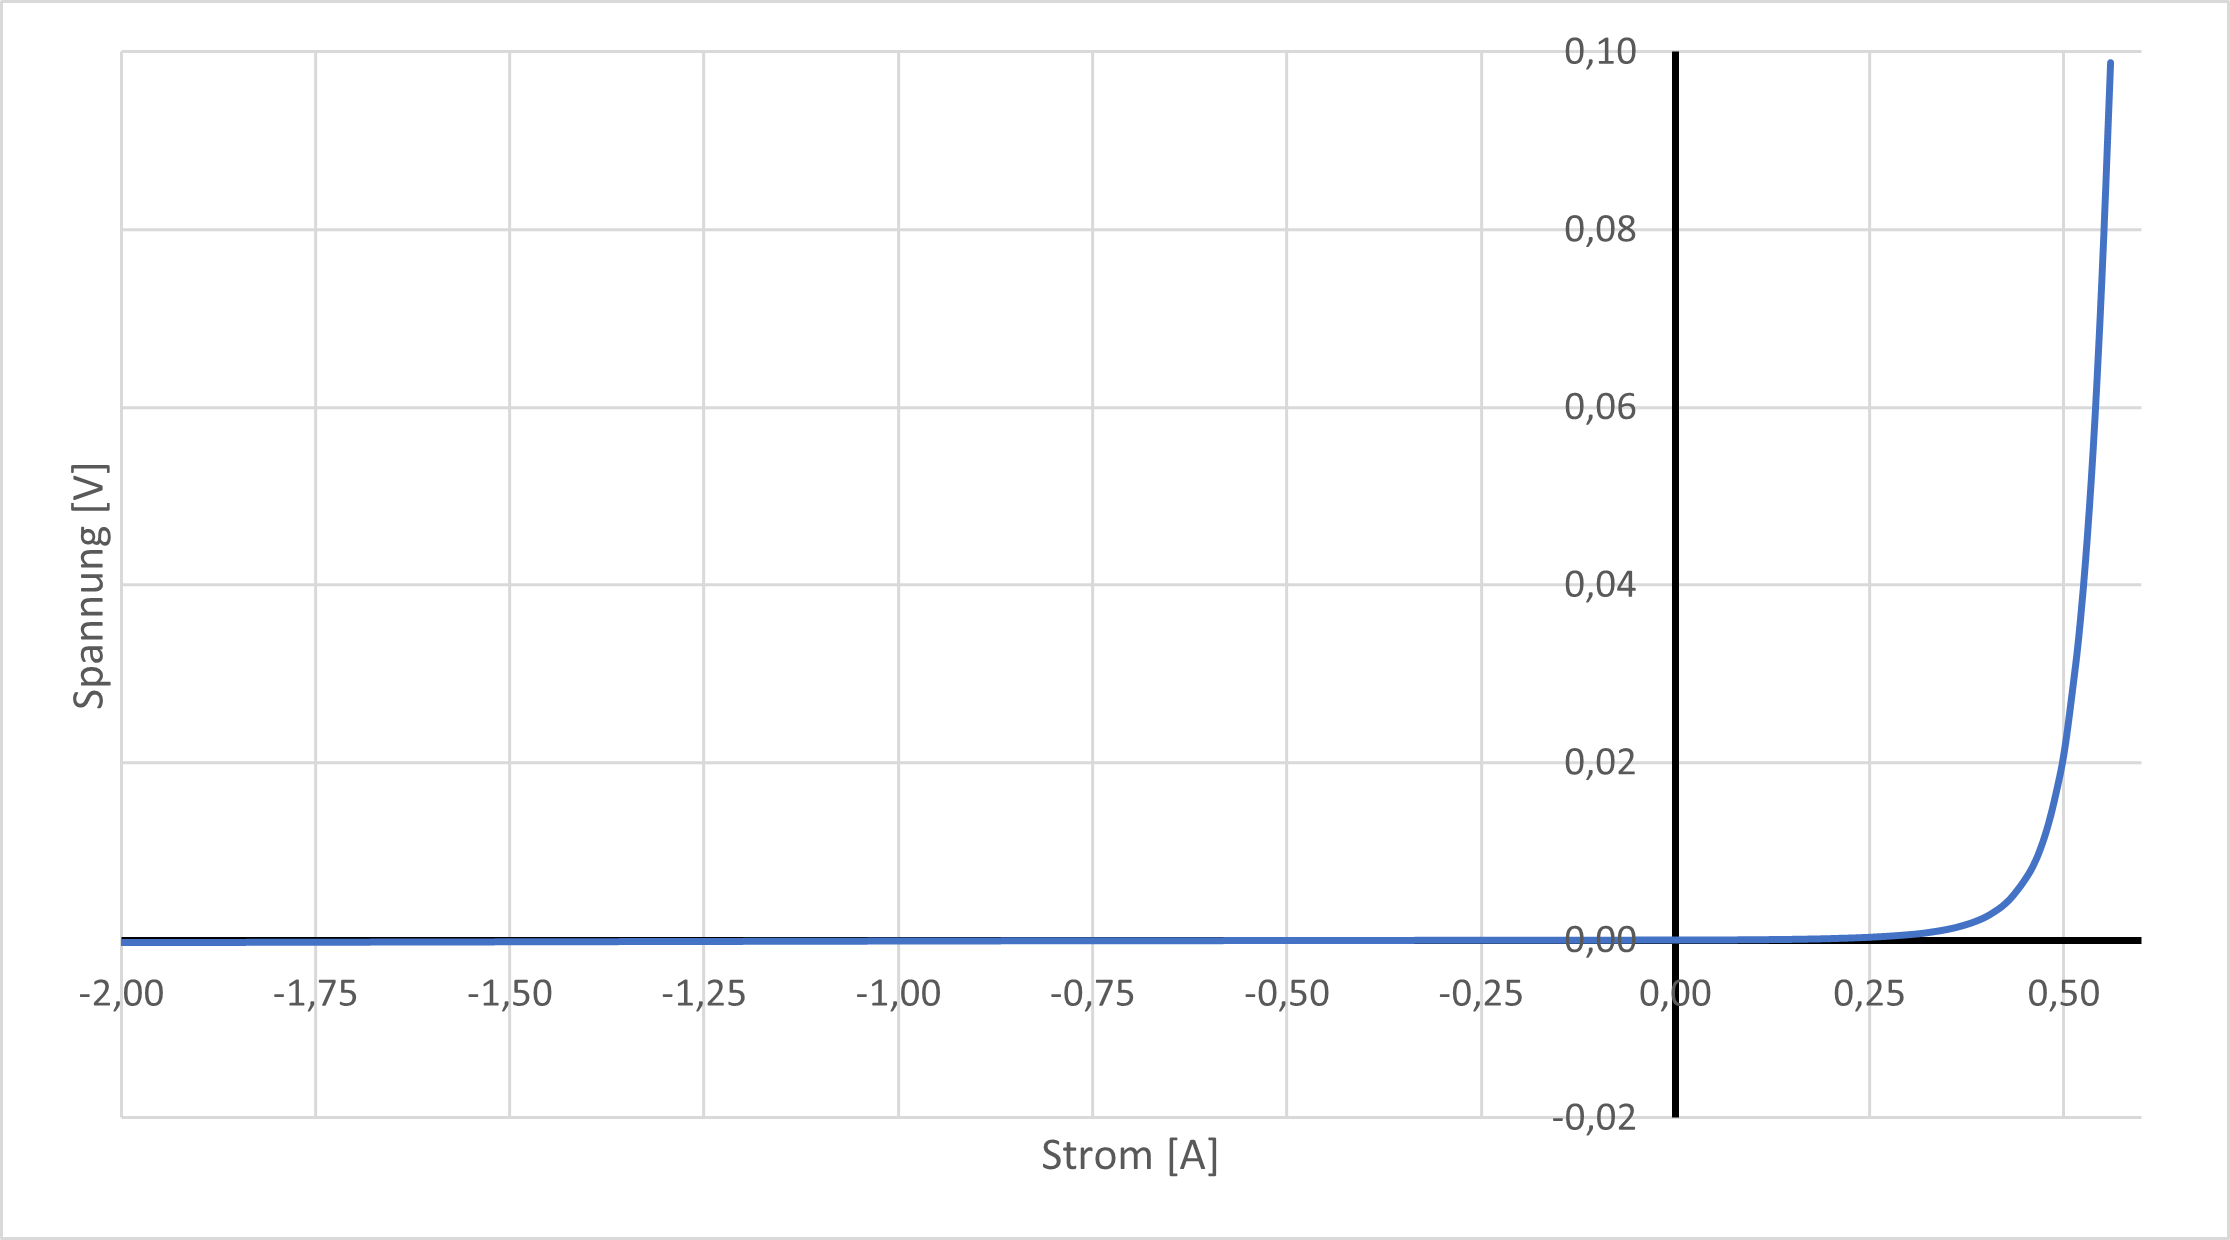
\includegraphics[width=14cm]{Diagramm_unbeleuchtet}
\centering
\caption{Diagramm Solarzelle unbeleuchtet}
\centering
\end{figure}

\begin{table}[H]
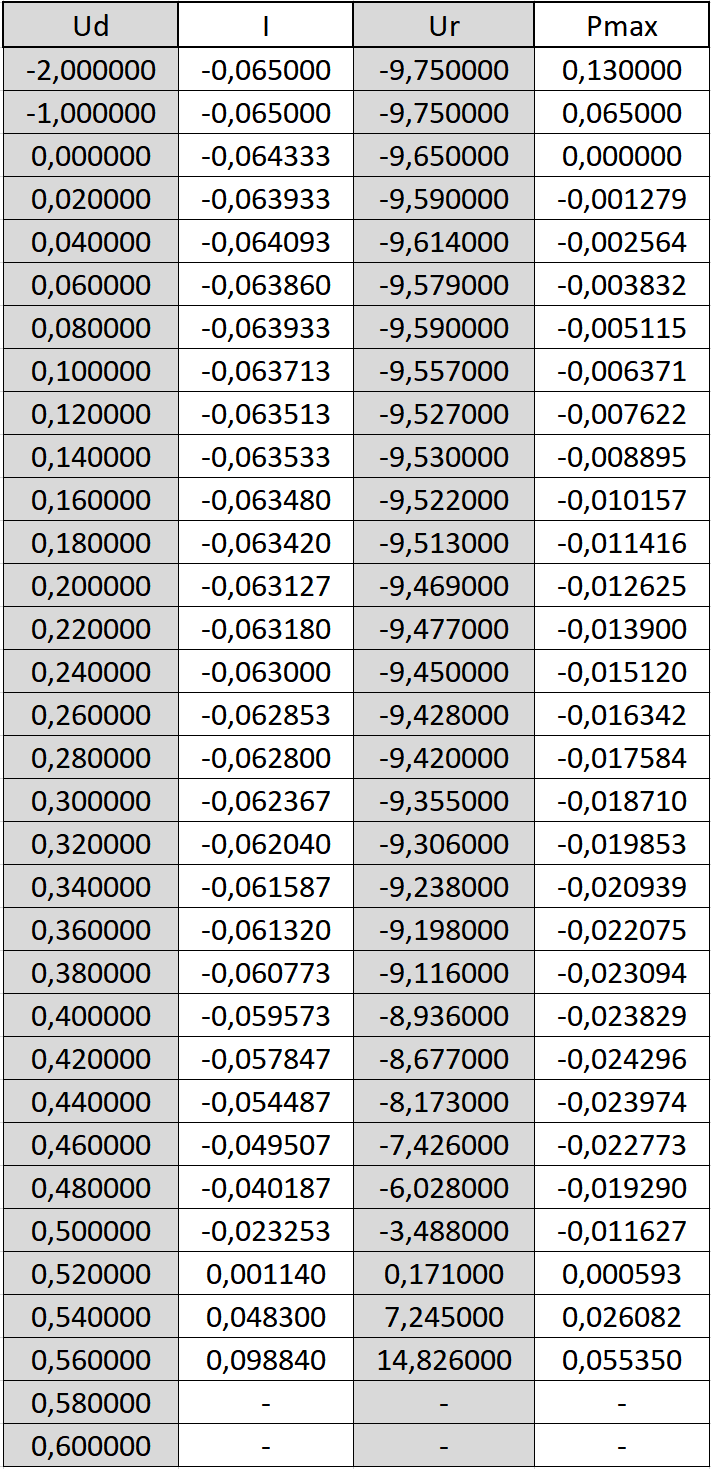
\includegraphics[width=6cm]{Tabelle_beleuchtet}
\centering
\caption{Messwerte Solarzelle unbeleuchtet}
\label{tab:beleuchtet}
\end{table}

\begin{figure}[H]
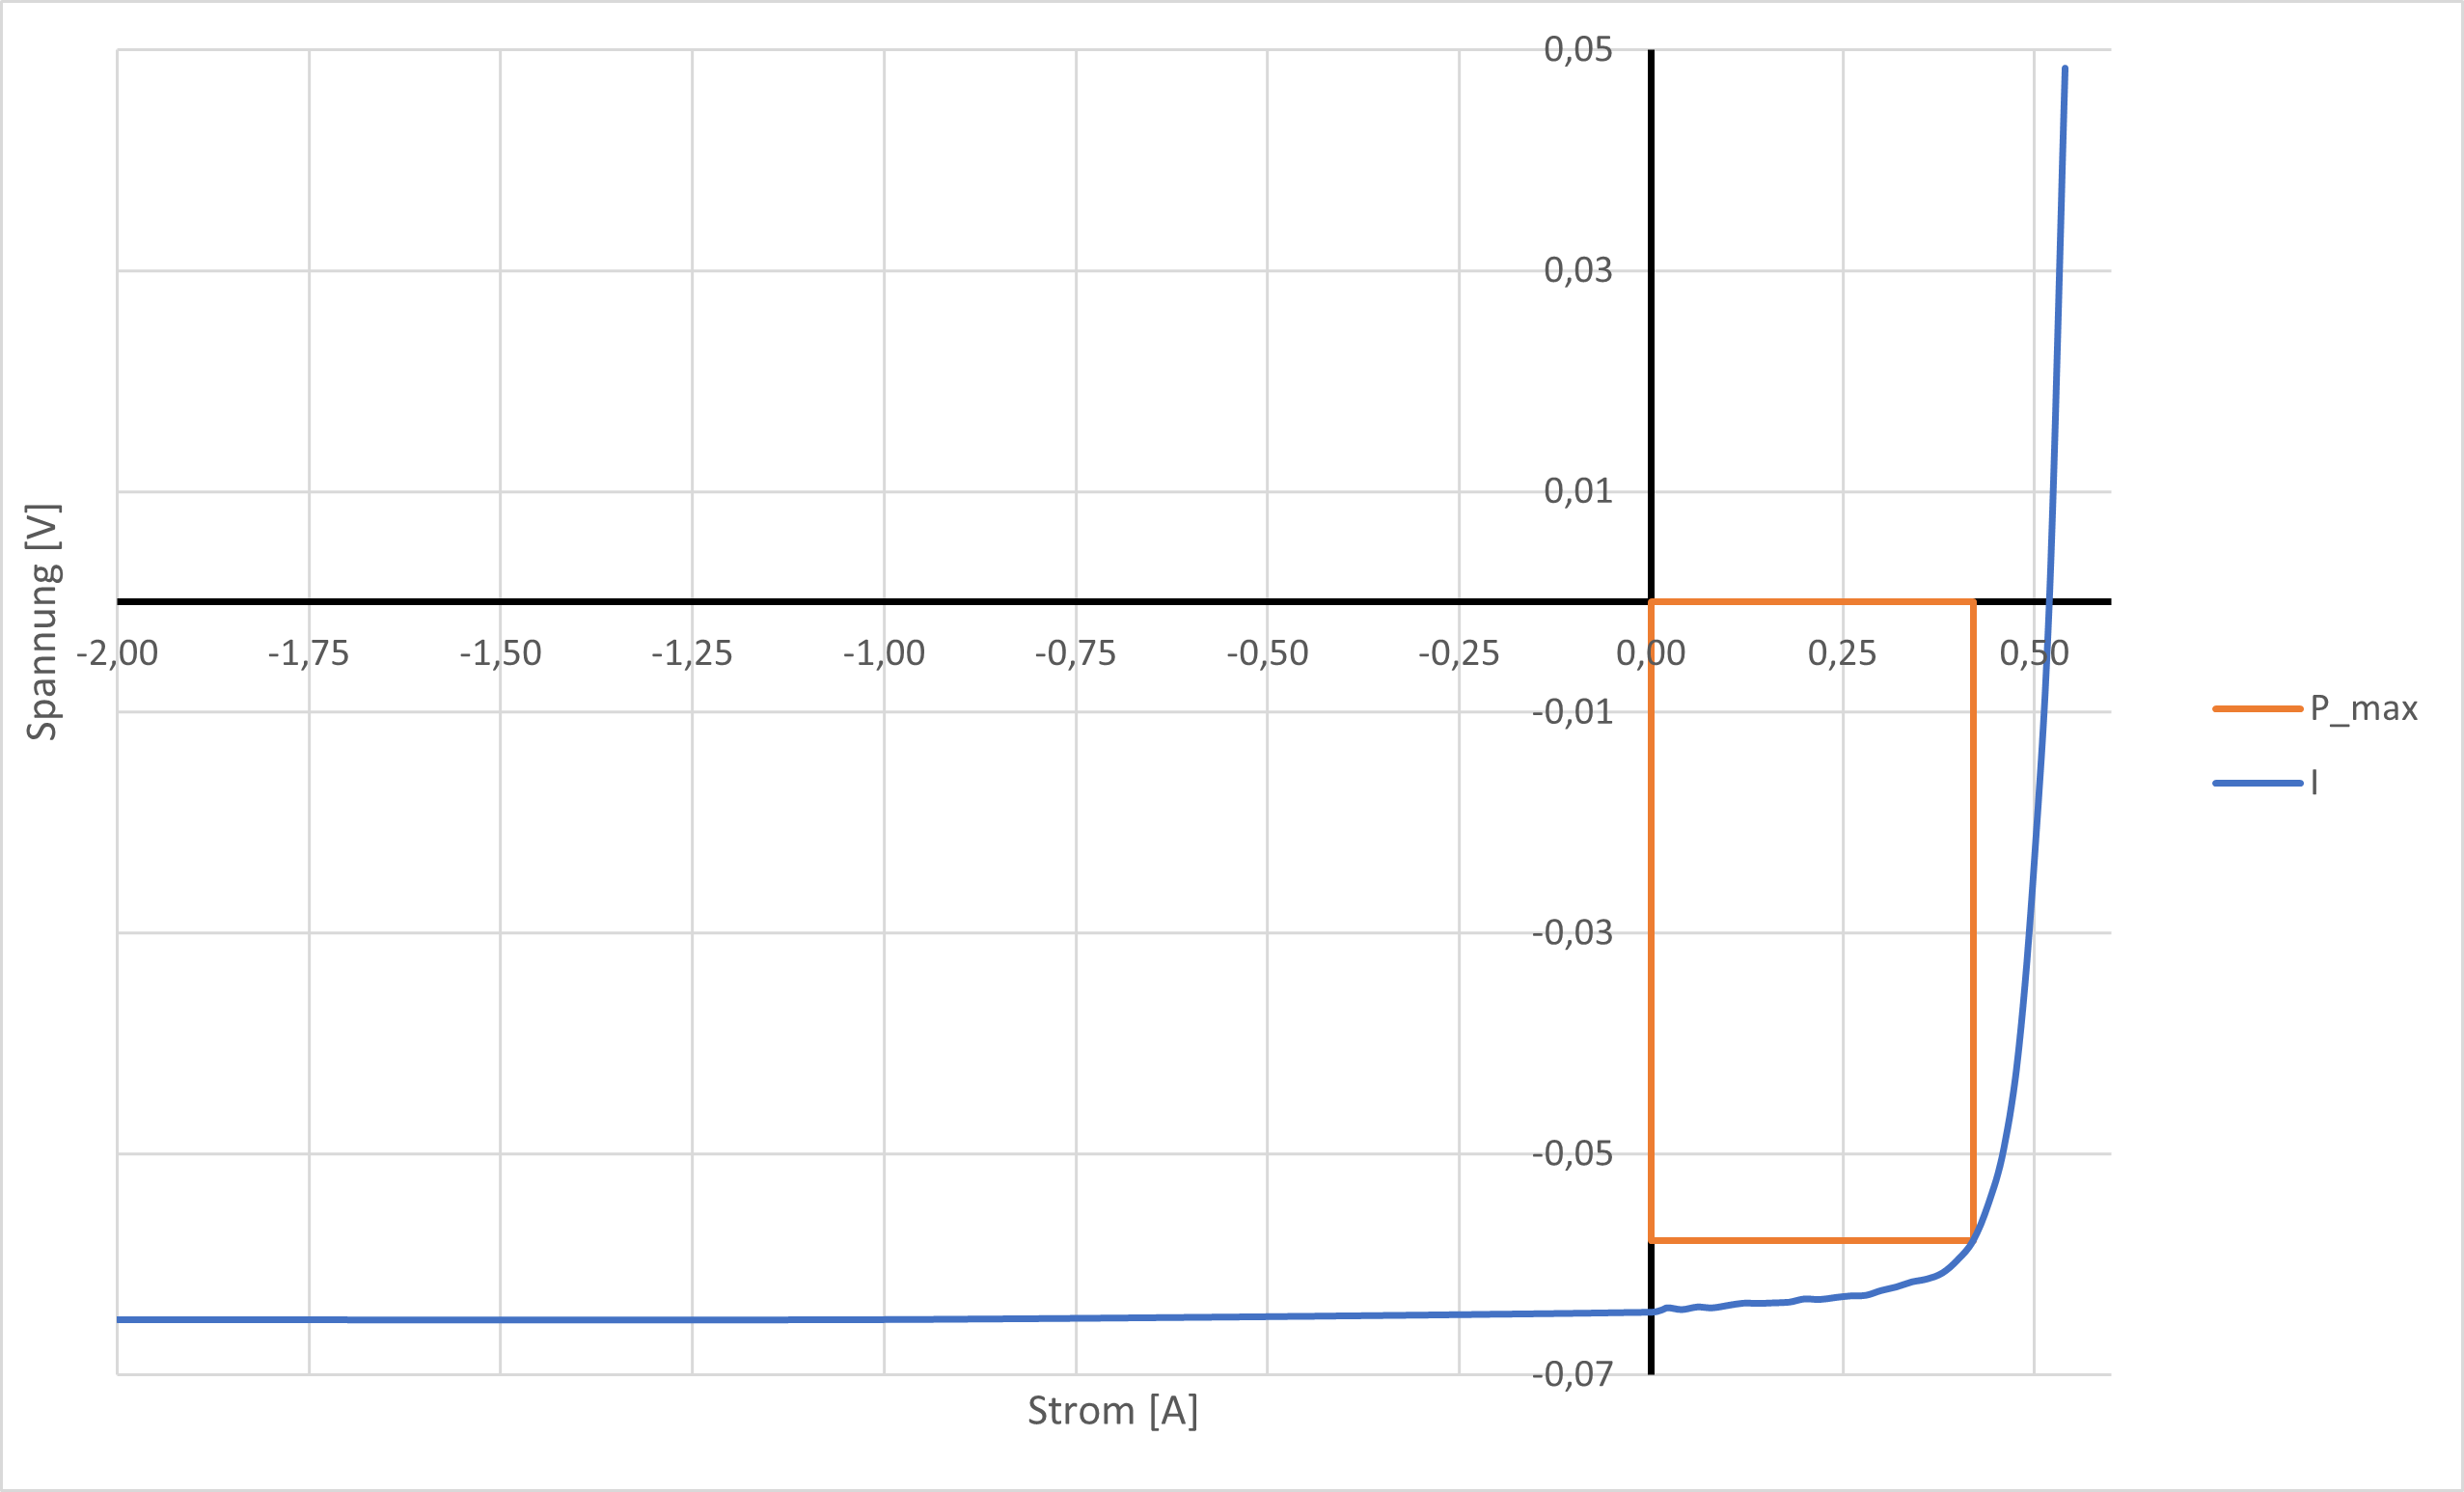
\includegraphics[width=14cm]{Diagramm_beleuchtet}
\centering
\caption{Diagramm Solarzelle unbeleuchtet}
\centering
\label{fig:beleuchtet}
\end{figure}

\newpage

\bibliography{literatur}




\label{LastPage}
\end{document}
%%% Local Variables:
%%% mode: latex
%%% TeX-master: t
%%% End: